\chapter{IMPLEMENTASI DAN PENGUJIAN}
\label{chapter:IMPLEMENTASI DAN PENGUJIAN}
\section{Implementasi}

\subsection{Struktur Antarmuka dan Modul Sistem}
\begin{enumerate}[label=\arabic*.]
    \item Modul Pemasaran \& Publik: menangani antarmuka awal dan etalase informasi aplikasi sebelum pengguna masuk:
    \begin{enumerate}[label=\alph*.]
        \item \texttt{LandingPage.tsx}: Halaman beranda interaktif dengan animasi roadmap dan efek kursor.
    \end{enumerate}
    
    \item Modul Autentikasi \& Manajemen Akun: menangani proses masuk, pendaftaran, serta pengaturan profil pengguna:
    \begin{enumerate}[label=\alph*.]
        \item \texttt{Login.tsx}, \texttt{Register.tsx}: Form login dan registrasi peran akun (Donatur, Penerima, Relawan).
        \item \texttt{ForgotPassword.tsx}: Antarmuka pemulihan kata sandi pengguna.
        \item \texttt{index.tsx}, \texttt{ProfileHeader.tsx}: Dashboard profil dan ringkasan gamifikasi level.
        \item \texttt{AIApiManagement.tsx}: Manajemen input Gemini API Key pribadi untuk membuka fitur AI lanjutan.
        \item \texttt{EditProfile.tsx}, \texttt{SecuritySettings.tsx}: Form pembaruan biodata dan keamanan akun.
        \item \texttt{AddressList.tsx}: Pengaturan titik koordinat alamat logistik.
        \item \texttt{ClaimHistory.tsx}, \texttt{ClaimHistoryDetail.tsx}: Riwayat klaim donasi makanan yang telah dilakukan pengguna.
        \item \texttt{PointHistory.tsx}, \texttt{GamificationSummary.tsx}: Catatan riwayat poin dan pencapaian gamifikasi pengguna.
        \item \texttt{FaqSection.tsx}, \texttt{SavedItems.tsx}: Pusat bantuan in-app dan daftar donasi yang disimpan.
    \end{enumerate}
    
    \item Modul Manajemen Donasi \& Gudang Makanan (Provider): digunakan oleh donatur untuk mengelola stok, donasi, dan riwayat pesanan:
    \begin{enumerate}[label=\alph*.]
        \item \texttt{index.tsx}: Dashboard utama logistik donatur.
        \item \texttt{Inventory.tsx}, \texttt{InventoryNavigation.tsx}: Menampilkan daftar makanan yang sedang tayang di platform.
        \item \texttt{QualityCheckInventoryInput.tsx}: Form unggah donasi pangan dengan fitur Live Camera.
        \item \texttt{QualityCheckInventory.tsx}: Memproses audit kelayakan donasi makanan menggunakan AI Gemini.
        \item \texttt{CorporateAIWidgets.tsx}: Widget AI khusus (Kreator Resep, CSR Writer) untuk donatur korporat.
        \item \texttt{ImpactWidget.tsx}, \texttt{QuickActions.tsx}, \texttt{StatsGrid.tsx}, \texttt{RankCard.tsx}: Kumpulan widget statistik pada dashboard donatur.
        \item \texttt{StockManager.tsx}, \texttt{StockFilters.tsx}, \texttt{ProductDetailModal.tsx}: Manajemen daftar stok, filter, dan detail donasi.
        \item \texttt{OrderList/index.tsx}, \texttt{OrderItemCard.tsx}: Daftar pesanan atau klaim masuk dari penerima.
        \item \texttt{OrderDetail/index.tsx}, \texttt{CourierInfo.tsx}, \texttt{ReceiverInfo.tsx}, \texttt{TimelineDetails.tsx}: Detail proses logistik dan status pengiriman pesanan donasi.
        \item \texttt{HistoryList/index.tsx}, \texttt{HistoryItemCard.tsx}, \texttt{HistoryDetail/index.tsx}, \texttt{Timeline.tsx}: Daftar dan detail riwayat donasi yang telah selesai (riwayat logistik).
        \item \texttt{Reports/index.tsx}, \texttt{ReportDetailModal.tsx}: Manajemen laporan dan komplain dari pengguna terkait donasi.
        \item \texttt{Reviews/index.tsx}, \texttt{ReviewItemCard.tsx}: Menampilkan ulasan dan rating dari penerima donasi.
    \end{enumerate}

    \item Modul Radar Penerima (Receiver): menangani eksplorasi donasi makanan terdekat dan pusat permintaan bagi penerima:
    \begin{enumerate}[label=\alph*.]
        \item \texttt{index.tsx}: Dashboard eksplorasi utama bagi panti asuhan atau individu penerima manfaat.
        \item \texttt{FoodList.tsx}, \texttt{FoodDetail.tsx}: Menampilkan katalog visual donasi terdekat beserta jarak radius dan detailnya.
        \item \texttt{AIVerificationCard.tsx}: Komponen stempel hijau jaminan mutu bahwa donasi telah diaudit oleh AI.
        \item \texttt{StoreIcon.tsx}: Representasi visual ikon toko atau titik donatur di peta.
        \item \texttt{RequestManager.tsx}: Fasilitas bagi penerima untuk mempublikasikan permintaan donasi spesifik ke publik donatur.
    \end{enumerate}

    \item Modul Operasional Kurir \& Gamifikasi (Volunteer): digunakan oleh relawan untuk mengambil misi penjemputan dan melacak metrik operasional:
    \begin{enumerate}[label=\alph*.]
        \item \texttt{index.tsx}, \texttt{StatsDashboard.tsx}: Dashboard relawan yang memuat statistik harian (jarak tempuh dan poin).
        \item \texttt{MissionList.tsx}: Menampilkan daftar antrean misi penjemputan donasi yang tersedia untuk diambil.
        \item \texttt{MissionDetail.tsx}: Detail eksekusi misi yang mencakup manifest muatan, peta rute Google Maps 3-titik, fitur chat WA instan, dan QR Code Pickup.
        \item \texttt{HistoryList.tsx}: Log riwayat misi logistik pengantaran yang pernah diselesaikan.
        \item \texttt{Leaderboard.tsx}: Papan klasemen persaingan poin antar relawan.
    \end{enumerate}

    \item Modul Konfigurasi \& Intervensi Pusat (Admin): memiliki akses untuk mengelola gamifikasi, konten, logistik global, dan moderasi pengguna:
    \begin{enumerate}[label=\alph*.]
        \item \texttt{index.tsx}, \texttt{Overview.tsx}: Dashboard utama pengawas super-admin.
        \item \texttt{SystemConfig.tsx}, \texttt{LogViewer.tsx}: Pengaturan variabel sistem dan pemantauan aliran log teknis.
        \item \texttt{AdminList.tsx}, \texttt{Impact.tsx}: Manajemen data pengguna admin dan kalkulasi SROI (Social Return on Investment).
        \item \texttt{RanksManagement.tsx}: Mengelola level dan poin gamifikasi dengan antarmuka drag-and-drop.
        \item \texttt{Distribution.tsx}, \texttt{Moderation.tsx}: Pelacakan riwayat distribusi logistik lintas pengguna dan pemrosesan sengketa/komplain.
        \item \texttt{ContentCMS.tsx}: Sistem manajemen konten FAQ dan SOP menggunakan editor markdown.
        \item \texttt{Communication/index.tsx}, \texttt{BroadcastHistory.tsx}, \texttt{ComposeMessage.tsx}: Mengelola pengiriman siaran pesan massal dari admin ke perangkat pengguna.
        \item \texttt{Community/index.tsx}, \texttt{UserList.tsx}, \texttt{VerificationModal.tsx}: Manajemen daftar pengguna dan verifikasi keabsahan institusi yayasan/restoran.
        \item \texttt{Community/BadgeCatalog.tsx}, \texttt{BadgeModal.tsx}: Mengelola pembuatan katalog medali/badge pencapaian untuk pengguna.
    \end{enumerate}

    \item Modul Penunjang Bersama (Shared Components): berisi elemen antarmuka, utilitas AI, dan pop-up yang dipakai lintas modul di atas:
    \begin{enumerate}[label=\alph*.]
        \item \texttt{DesktopLayout.tsx}, \texttt{Sidebar.tsx}, \texttt{TopAppBar.tsx}: Kerangka dan kerangka struktur navigasi utama aplikasi.
        \item \texttt{CSRWriterEditor.tsx}, \texttt{EcoPackagingEditor.tsx}: Antarmuka editor cerdas bantuan AI.
        \item \texttt{KitchenScanner.tsx}: Modul integrasi pemindai kamera untuk kelayakan fasilitas dapur.
        \item \texttt{AddressWarningModal.tsx}, \texttt{VerificationPendingModal.tsx}, \texttt{SuccessClaimSplash.tsx}: Kumpulan modal peringatan dan notifikasi splash (pop-up sistem).
        \item \texttt{Button.tsx}, \texttt{Input.tsx}, \texttt{CounterUp.tsx}: Blok pembangun dasar UI sistem (komponen form, tombol, dan animasi numerik).
    \end{enumerate}
\end{enumerate}

\subsection{Hak Akses Pengguna (\textit{Role-Based Access Control})}

Kapasitas jumlah pengguna pada platform FoodAI Rescue tidak dibatasi secara kuantitas, namun kewenangannya diklasifikasikan ke dalam 6 (enam) jenis peran yang berbeda untuk menjaga keamanan dan privasi data. Keenam jenis pengguna tersebut adalah:

\begin{enumerate}[label=\arabic*.]
    \item \textbf{Donatur Individu}: Pengguna skala rumah tangga atau usaha mikro yang dapat mengunggah donasi makanan sisa, memantau Dasbor Dampak Sosial (SROI), serta menggunakan AI \textit{Quality Verification} ("Polisi Pangan") untuk memvalidasi kelayakan makanan secara mandiri.
    \item \textbf{Donatur Korporat}: Pengguna dari sektor industri komersial (HORECA) yang memiliki fungsionalitas serupa dengan donatur individu, ditambah hak akses eksklusif terhadap modul AI Generatif (\textit{Eco Packaging Editor} dan \textit{CSR Copywriter}) guna memproduksi materi kampanye keberlanjutan perusahaan.
    \item \textbf{Penerima (Mitra Penerima)}: Kelompok masyarakat rentan atau fasilitas sosial yang memiliki akses untuk mencari ketersediaan makanan di radar peta, melakukan klaim (\textit{booking}) pesanan, serta memberikan ulasan pasca-donasi.
    \item \textbf{Relawan (Kurir Logistik)}: Pasukan sukarela yang bertugas mengambil misi penjemputan dan pengantaran makanan. Relawan berinteraksi dengan sistem menggunakan kewajiban pindai (\textit{mandatory scan}) Kode QR saat serah terima, dan berhak mendapatkan poin XP pada sistem gamifikasi.
    \item \textbf{Admin Pengelola}: Pengelola sistem operasional yang bertugas memverifikasi pendaftaran akun, menangani laporan keluhan pengguna, memantau Dasbor Statistik, serta menyesuaikan parameter \textit{Prompt Engineering} pada AI.
    \item \textbf{Super Admin}: Tim pengembang (IT) yang memiliki kedaulatan penuh terhadap infrastruktur \textit{backend}, bertugas melakukan pemeliharaan server (mengaktifkan \textit{maintenance mode}), serta memonitor jejak \textit{log} sistem secara keseluruhan.
\end{enumerate}

\subsection{Langkah Instalasi dan Konfigurasi Sistem}
Untuk menginstal dan menjalankan platform FoodAI Rescue secara lokal (\textit{localhost}), langkah-langkah berikut dapat diikuti:

\begin{enumerate}[label=\arabic*.]
    \item Unduh (\textit{clone}) \textit{source code} aplikasi dari repositori GitHub dan buka proyek tersebut menggunakan IDE (misalnya Visual Studio Code).
    \item Siapkan dan aktifkan layanan basis data MySQL melalui panel kontrol XAMPP atau Laragon.
    \item Jalankan server \textit{backend} (arahkan terminal ke folder \texttt{server} lalu ketik \texttt{npm run dev}) dan berikan izin saat muncul peringatan untuk melakukan migrasi \textit{database} secara otomatis.
    \item Lakukan konfigurasi akun utama melalui terminal dengan memasukkan \textit{email} dan \textit{password} untuk \textit{Super Admin}, lalu \textit{scan} QR Code untuk menautkan layanan \textit{gateway} WhatsApp.
    \item Jalankan server \textit{frontend} (buka terminal baru pada direktori utama lalu ketik \texttt{npm run dev}).
    \item Akses dan jalankan sistem melalui peramban (\textit{web browser}) pada alamat \url{http://localhost:3000/}.
\end{enumerate}

\subsection{User Manual}

\textbf{A. Akses Pengguna}

\subsubsection{Proses Registrasi Pengguna}
Langkah-langkah untuk melakukan pendaftaran akun baru pada platform Food AI Rescue adalah sebagai berikut:
\begin{enumerate}[label=\arabic*.]
    \item Akses halaman utama aplikasi dan tekan tombol \textbf{Daftar Gratis}.
    \item Pilih peran (\textit{role}) pengguna yang sesuai dengan entitas Anda, misalnya Donatur, Penerima, atau Relawan.
    \item Isi kelengkapan formulir pendaftaran akun (seperti nama, email, dan kata sandi), lalu tekan \textbf{Daftar}.
    \item Masukkan kode OTP (\textit{One-Time Password}) yang dikirimkan ke alamat email Anda untuk menyelesaikan proses verifikasi.
\end{enumerate}

\begin{figure}[H]
    \centering
    \includegraphics[width=\linewidth]{image/bab4/UserManual/Registrasi/1-Landing.png}
    \caption{Halaman Utama Aplikasi}
\end{figure}

\begin{figure}[H]
    \centering
    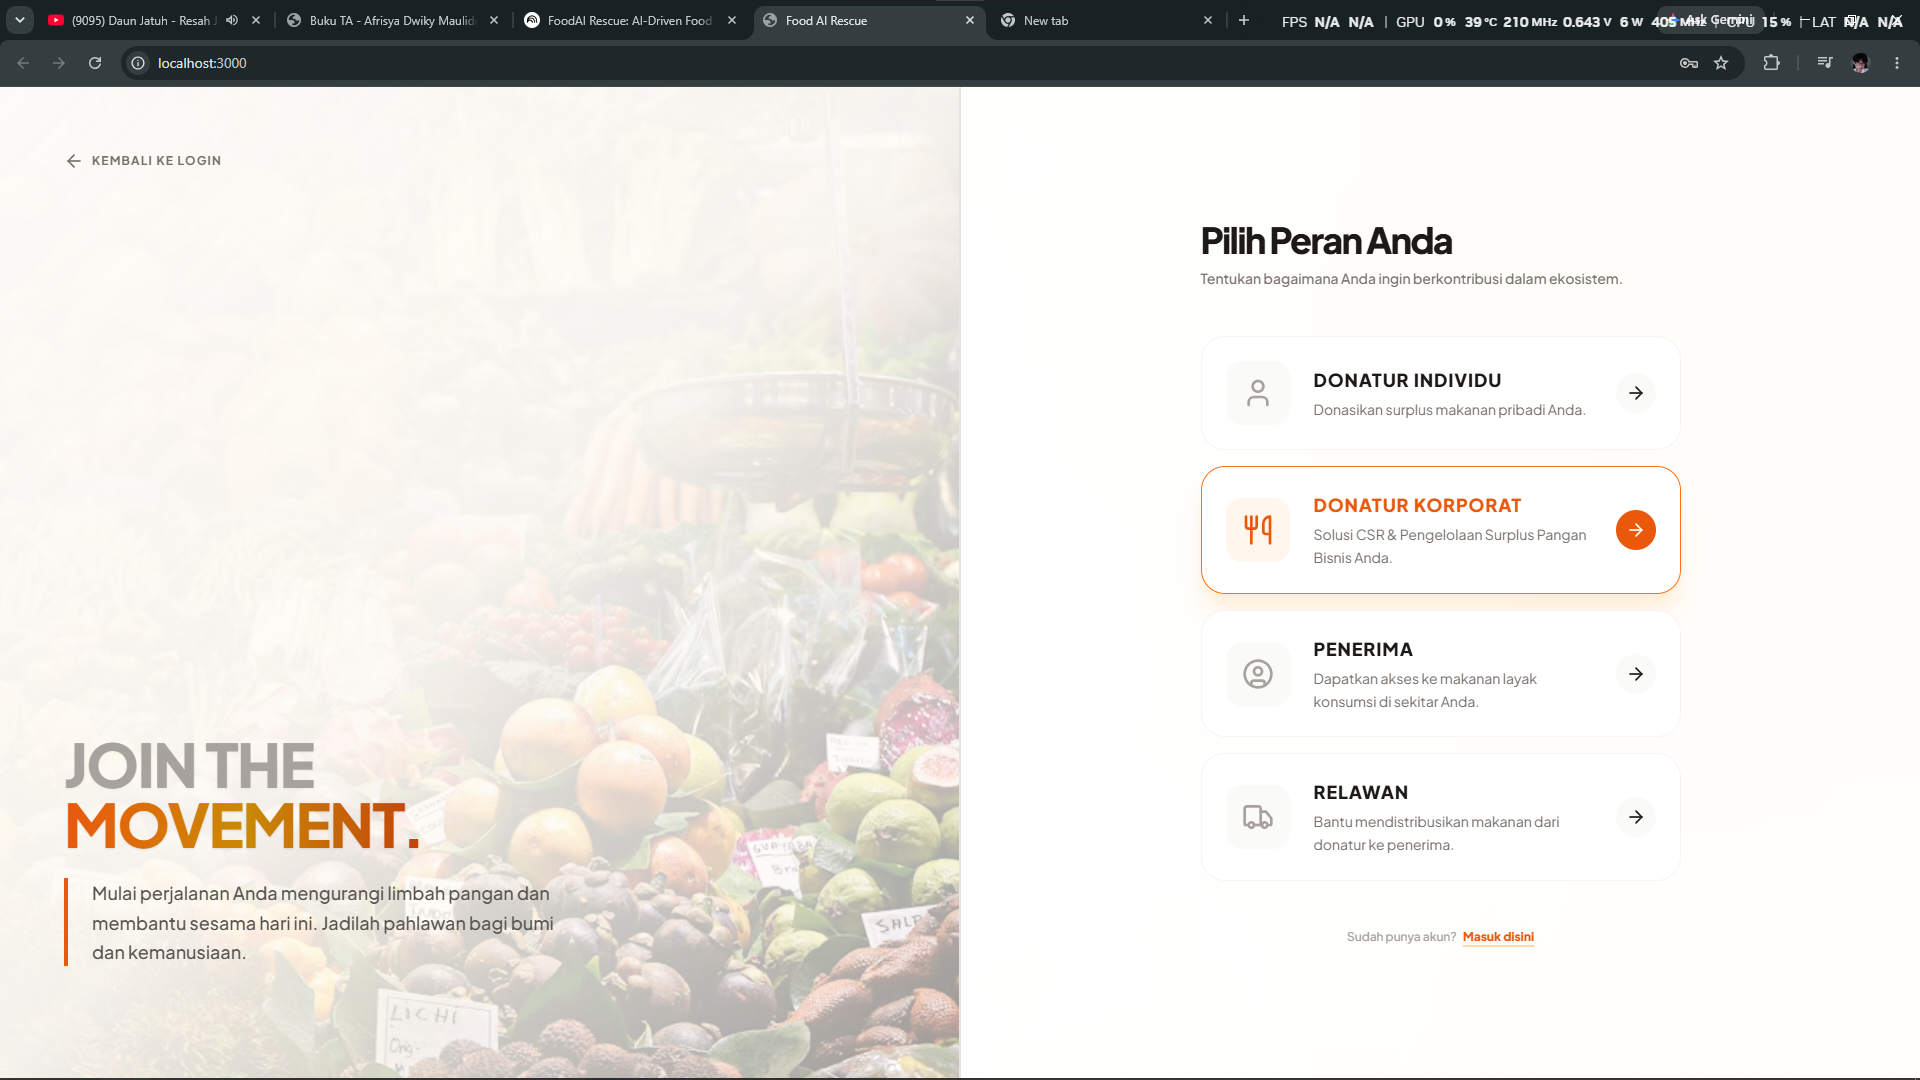
\includegraphics[width=\linewidth]{image/bab4/UserManual/Registrasi/2-PilihPeran.png}
    \caption{Halaman Pemilihan Peran}
\end{figure}



\begin{figure}[H]
    \centering
    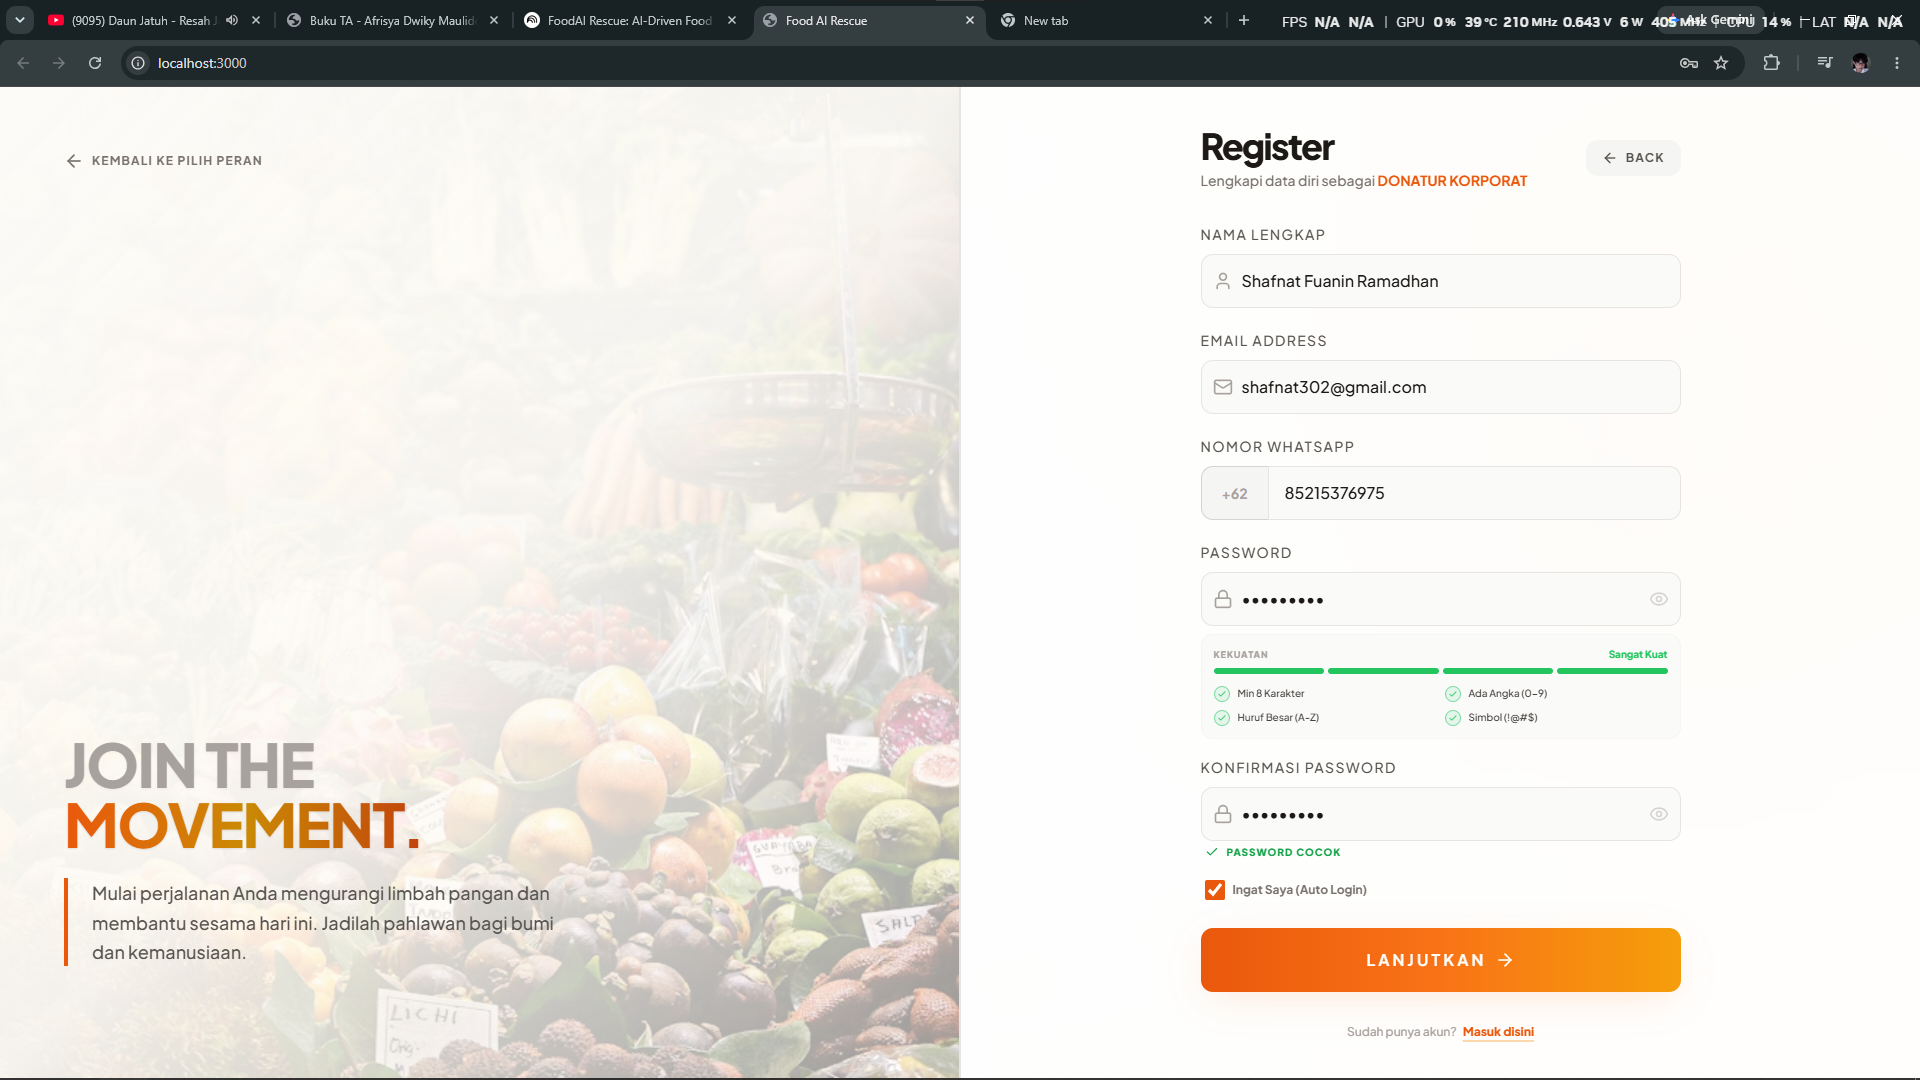
\includegraphics[width=\linewidth]{image/bab4/UserManual/Registrasi/3-Register.png}
    \caption{Formulir Registrasi}
\end{figure}

\begin{figure}[H]
    \centering
    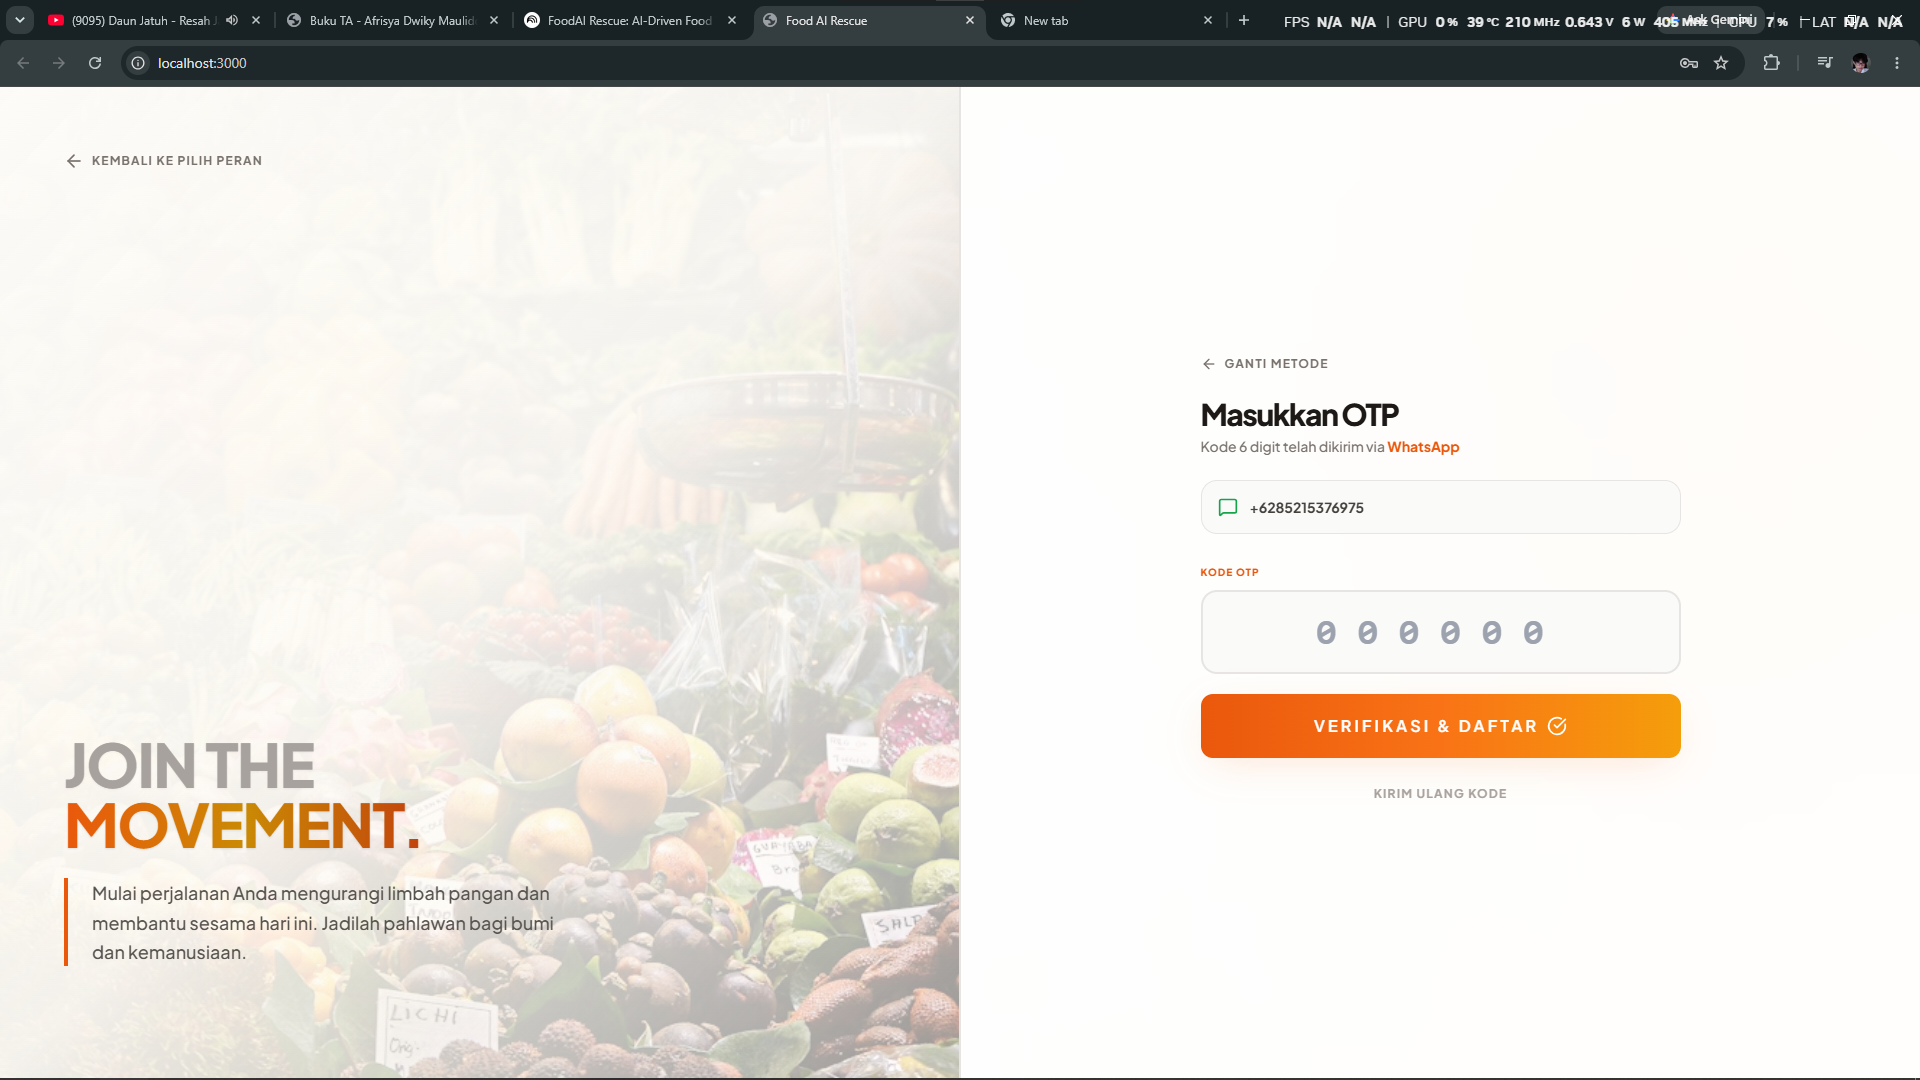
\includegraphics[width=\linewidth]{image/bab4/UserManual/Registrasi/4-OTP.png}
    \caption{Verifikasi OTP}
\end{figure}



\subsubsection{Proses Login Pengguna}
Langkah-langkah untuk masuk ke dalam dasbor sistem:
\begin{enumerate}[label=\arabic*.]
    \item Akses halaman utama dan tekan tombol \textbf{Masuk}.
    \item Masukkan kredensial email dan kata sandi yang telah terdaftar, kemudian tekan tombol \textbf{Masuk}.
\end{enumerate}

\begin{figure}[H]
    \centering
    \includegraphics[width=\linewidth]{image/bab4/UserManual/Login/1-Landing.png}
    \caption{Halaman Utama Aplikasi}
\end{figure}

\begin{figure}[H]
    \centering
    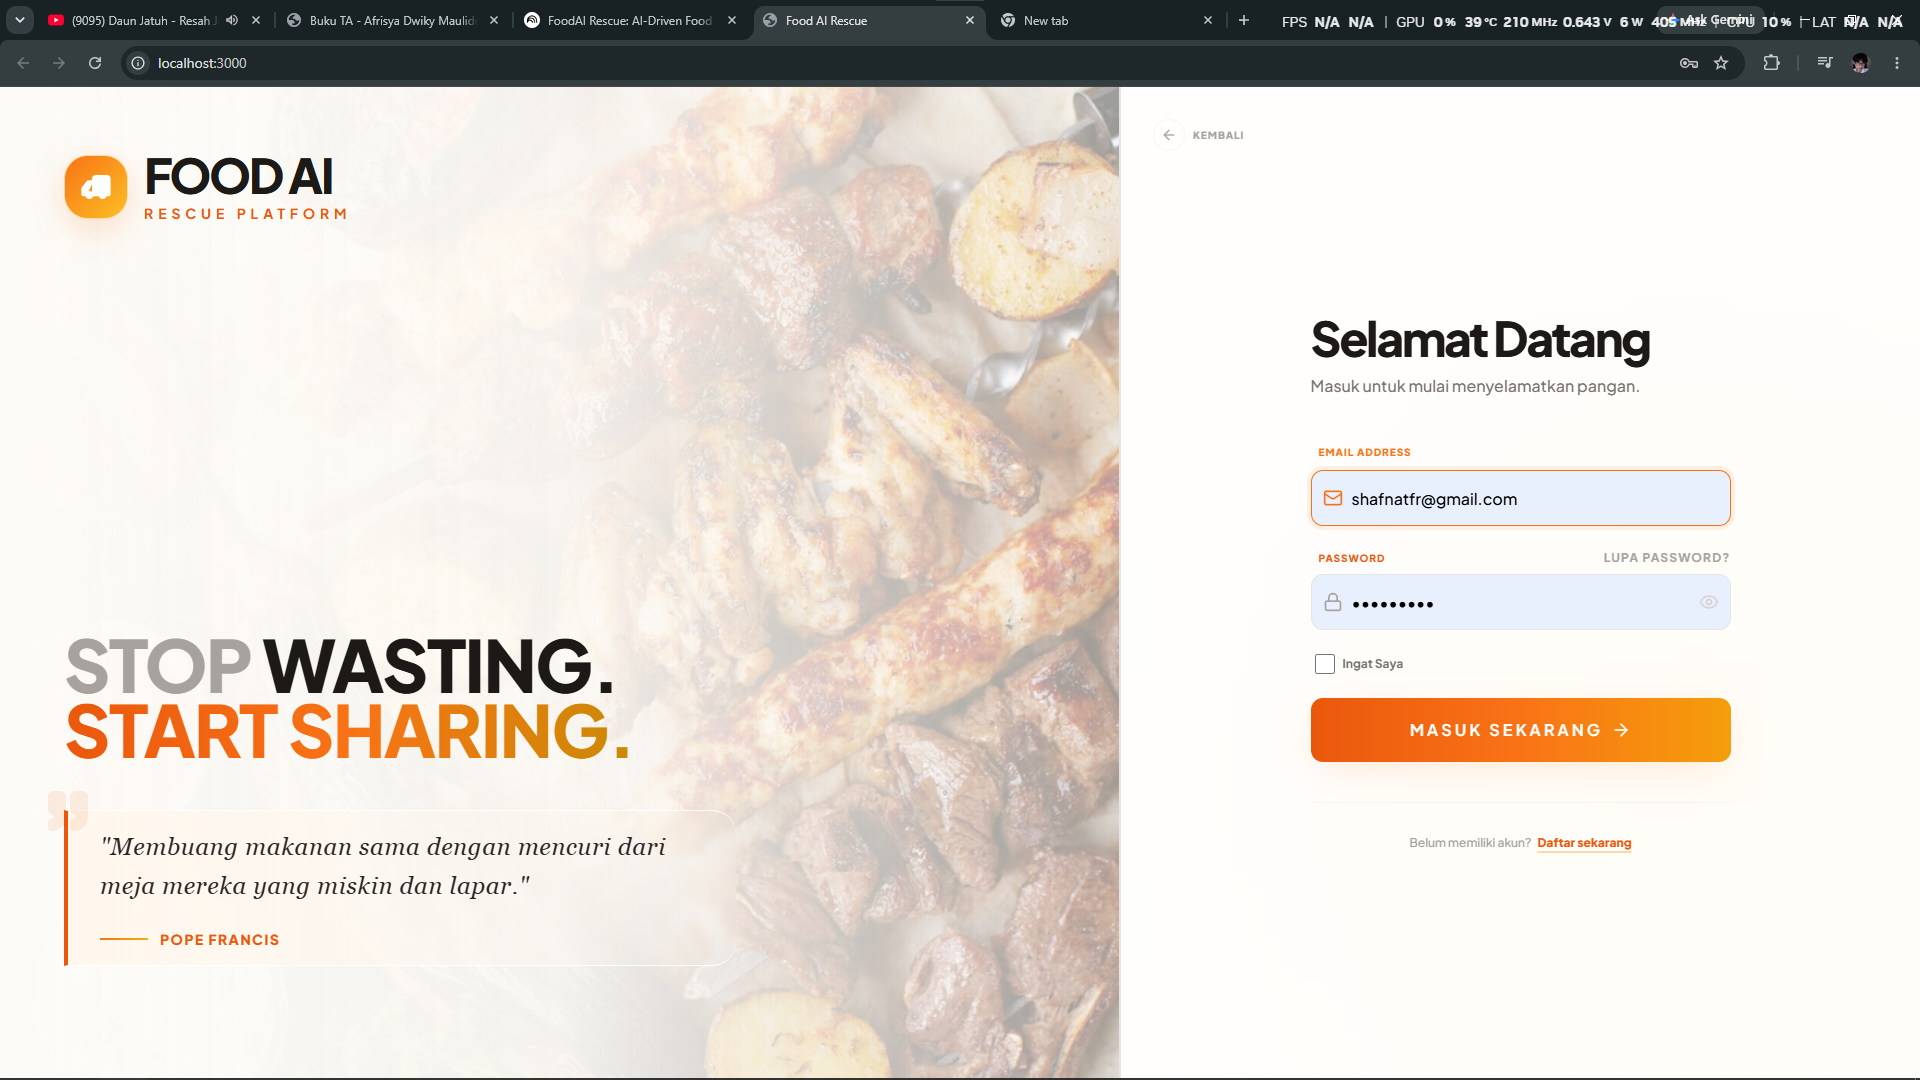
\includegraphics[width=\linewidth]{image/bab4/UserManual/Login/2-Login.png}
    \caption{Halaman \textit{Login}}
\end{figure}



\textbf{B. Pengguna Donatur (Penyedia Makanan)}

\subsubsection{Proses Input Donasi Makanan}
Langkah-langkah untuk mendata surplus makanan:
\begin{enumerate}[label=\arabic*.]
    \item Buka menu \textbf{Manajemen Stok} pada dasbor Donatur, lalu tekan \textbf{Tambah Donasi}.
    \item Isi rincian makanan yang akan didonasikan dan unggah fotonya.
    \item Sistem (Polisi Pangan) akan menampilkan hasil audit kualitas berbasis AI. Jika dinyatakan aman, tekan publikasikan donasi.
\end{enumerate}

\begin{figure}[H]
    \centering
    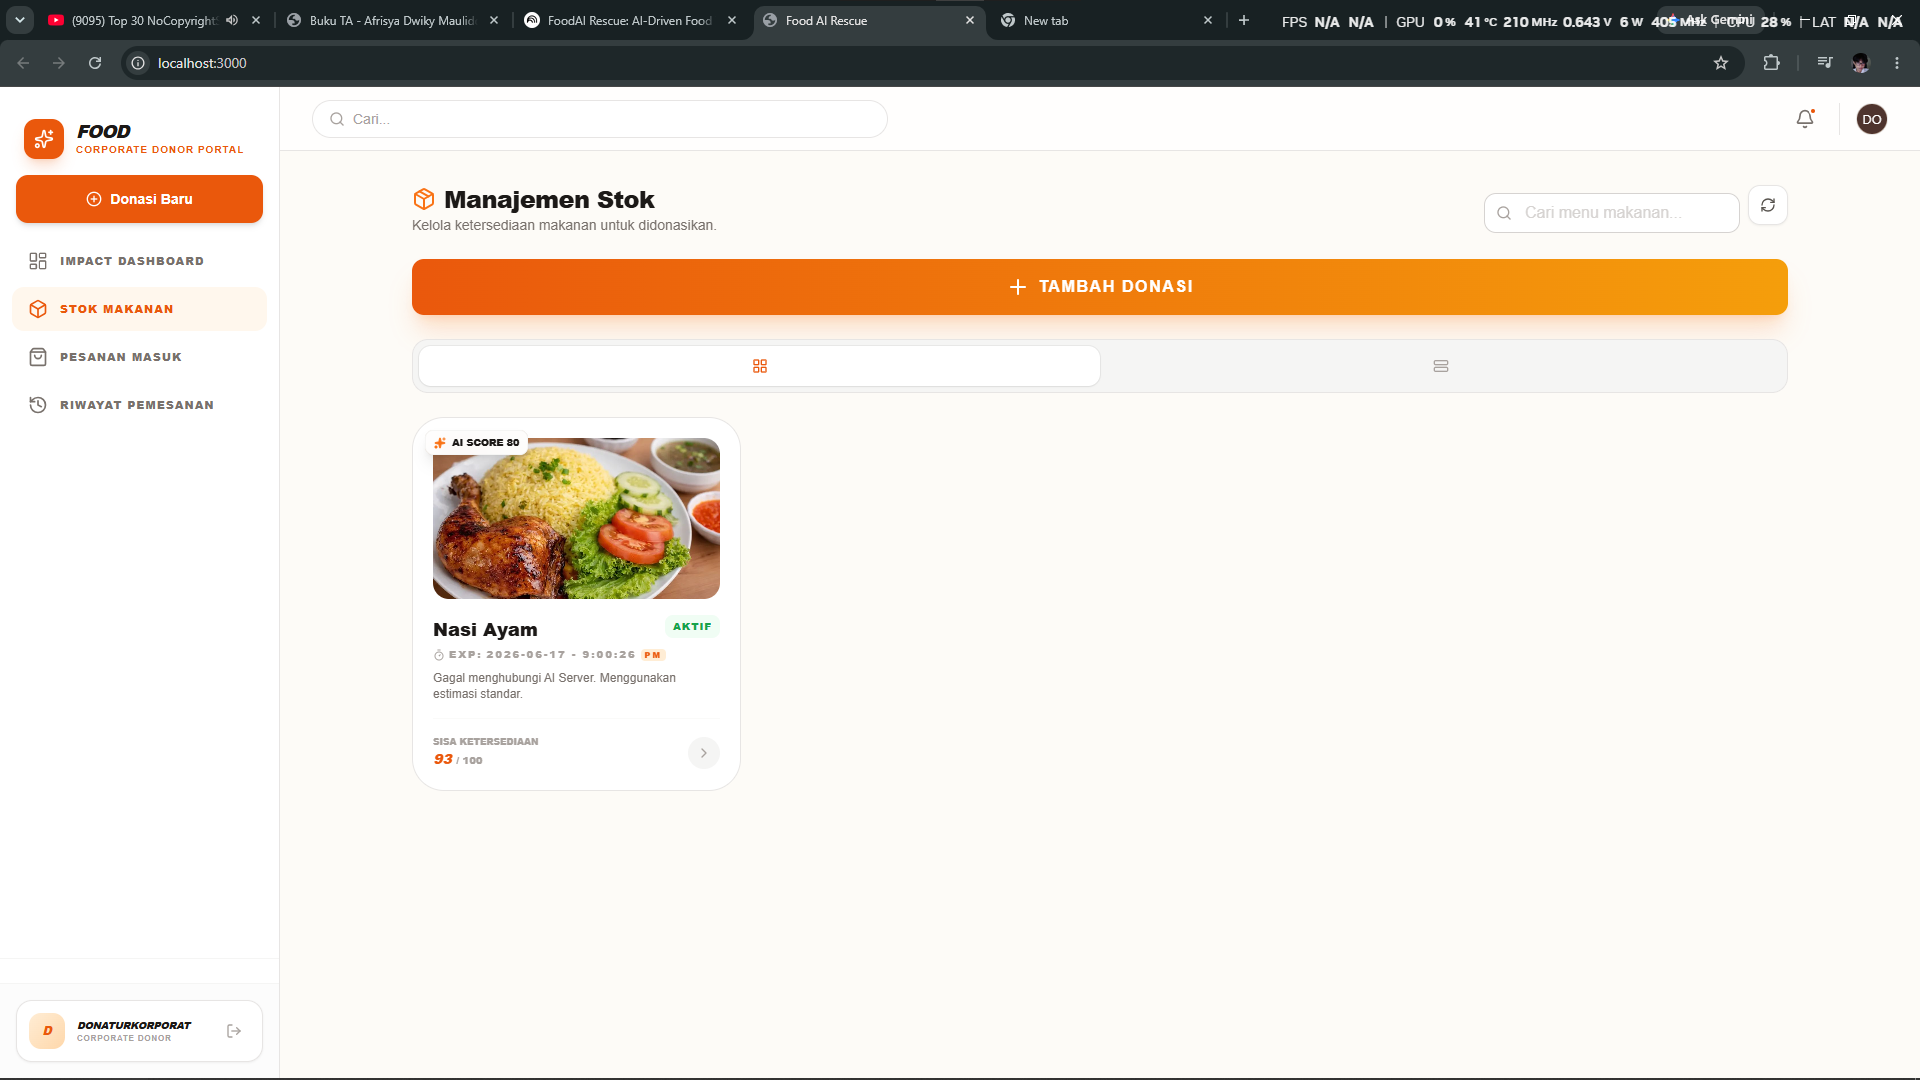
\includegraphics[width=\linewidth]{image/bab4/UserManual/InputDonasi/1-ManajemenStok.png}
    \caption{Manajemen Stok}
\end{figure}

\begin{figure}[H]
    \centering
    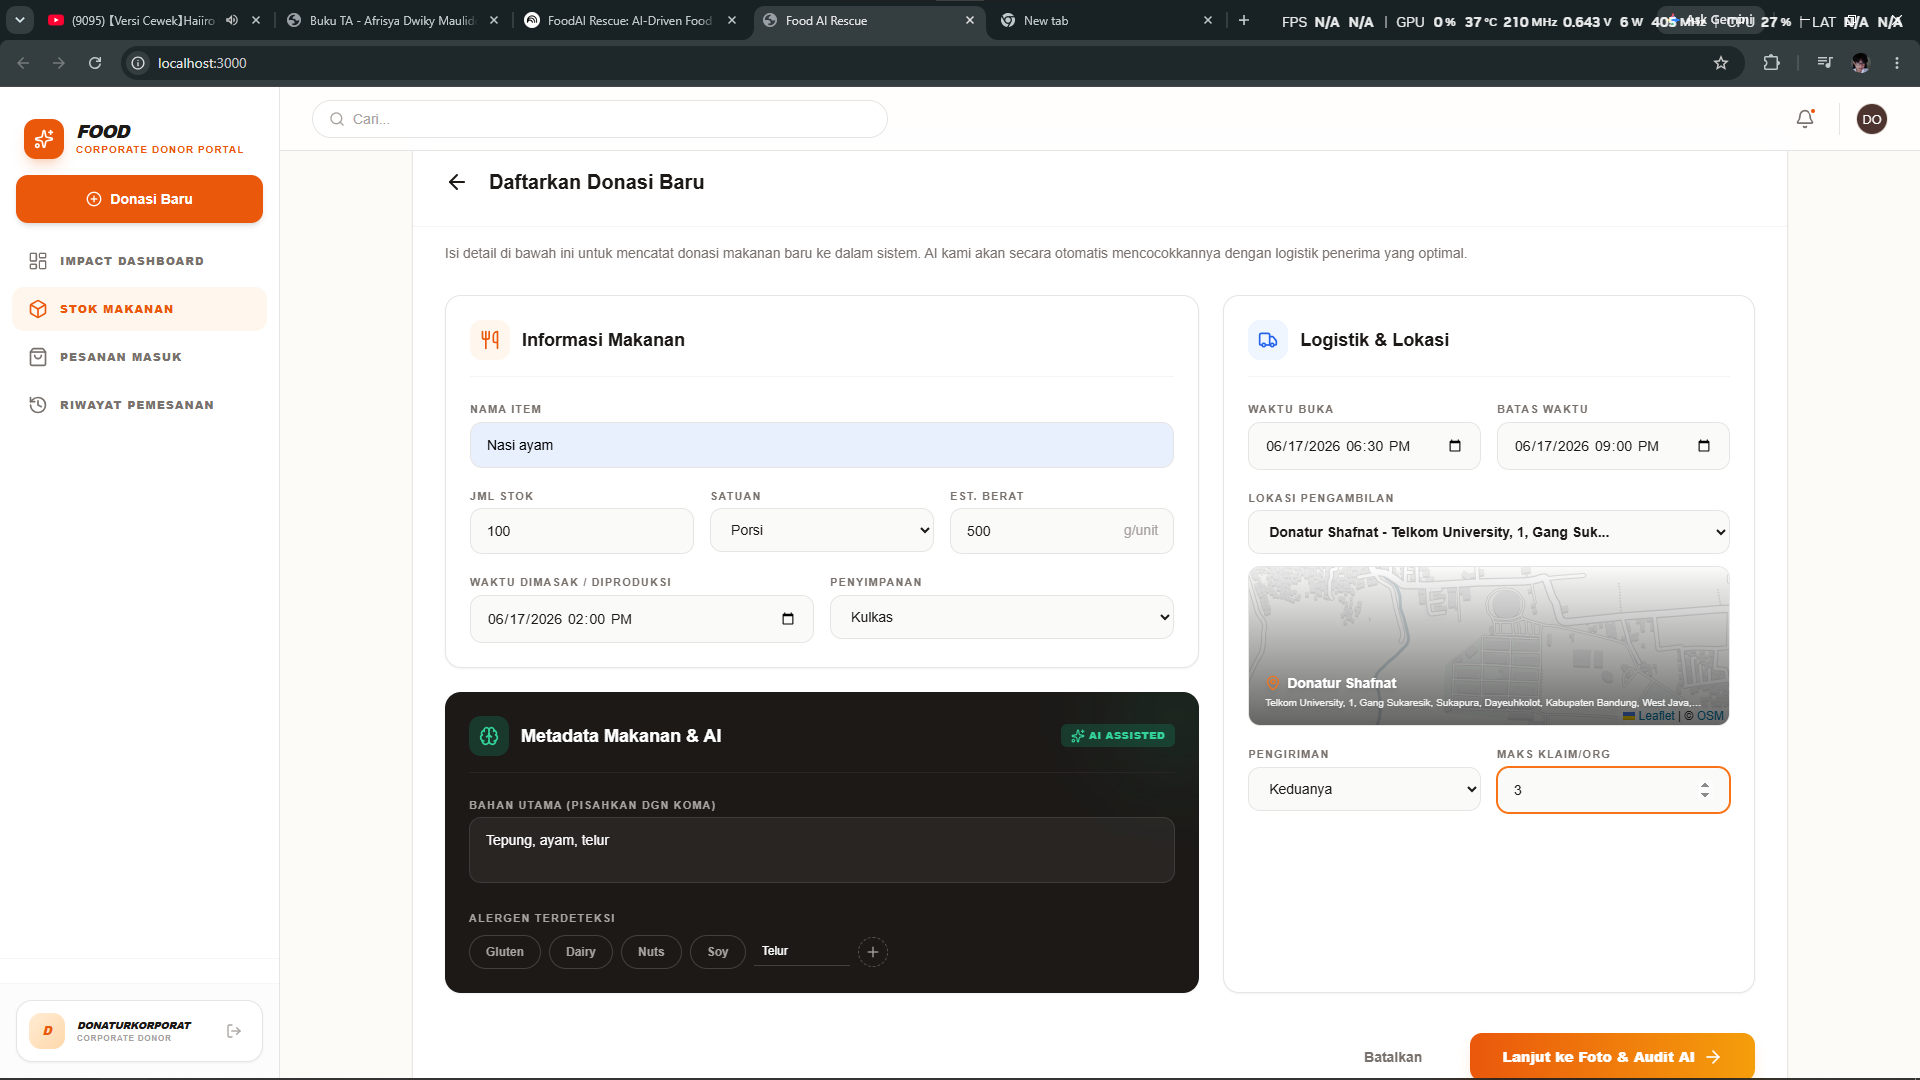
\includegraphics[width=\linewidth]{image/bab4/UserManual/InputDonasi/2-InputDataDonasi.png}
    \caption{Input Data Donasi}
\end{figure}

\begin{figure}[H]
    \centering
    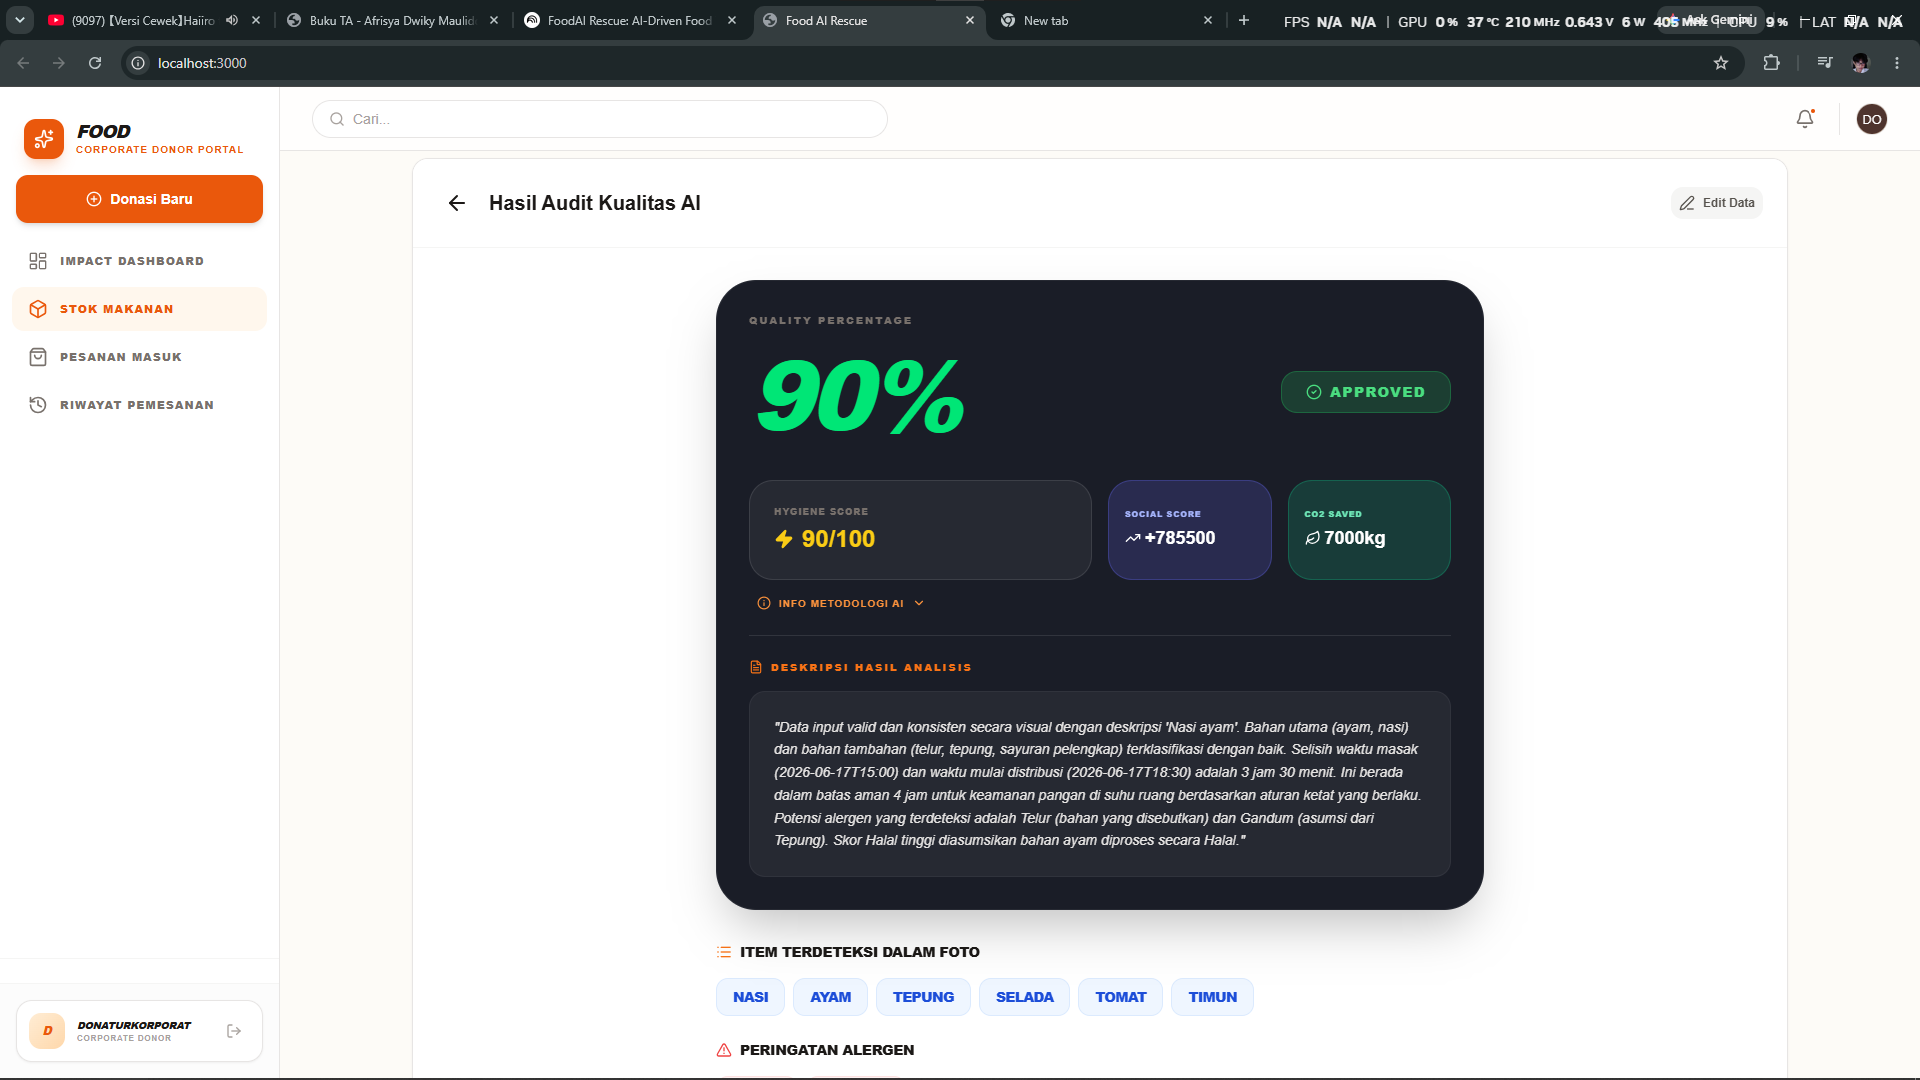
\includegraphics[width=\linewidth]{image/bab4/UserManual/InputDonasi/3-HasilAudit.png}
    \caption{Hasil Audit AI}
\end{figure}



\subsubsection{Proses Menerima dan Memproses Pesanan Masuk}
Langkah-langkah menerima pesanan dari penerima donasi:
\begin{enumerate}[label=\arabic*.]
    \item Buka menu \textbf{Pesanan Aktif} (Kelola Pesanan).
    \item Tekan pada pesanan yang masuk untuk melihat rincian (\textit{Detail Request}), lalu tekan setujui (\textit{Terima Request}).
\end{enumerate}

\begin{figure}[H]
    \centering
    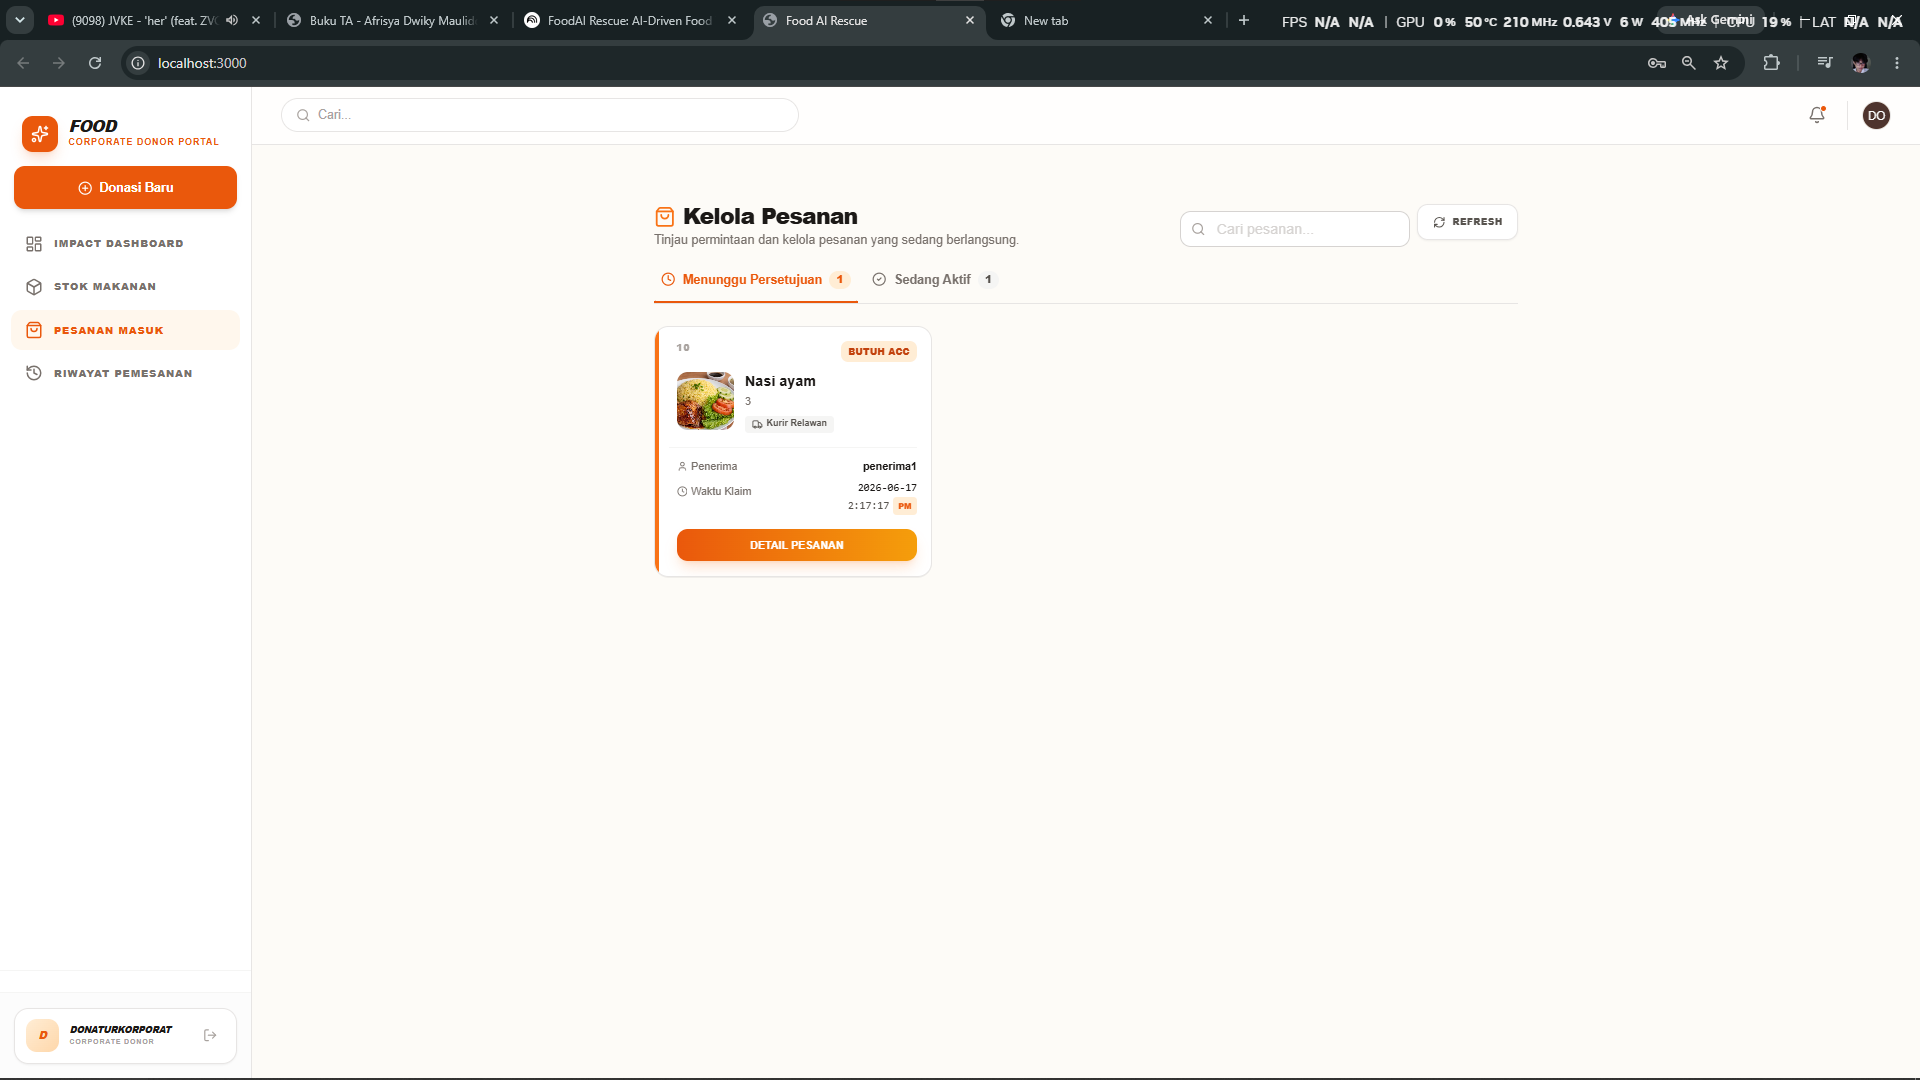
\includegraphics[width=\linewidth]{image/bab4/UserManual/TerimaPesanan/1-KelolaPesanan.png}
    \caption{Menu Pesanan Aktif}
\end{figure}

\begin{figure}[H]
    \centering
    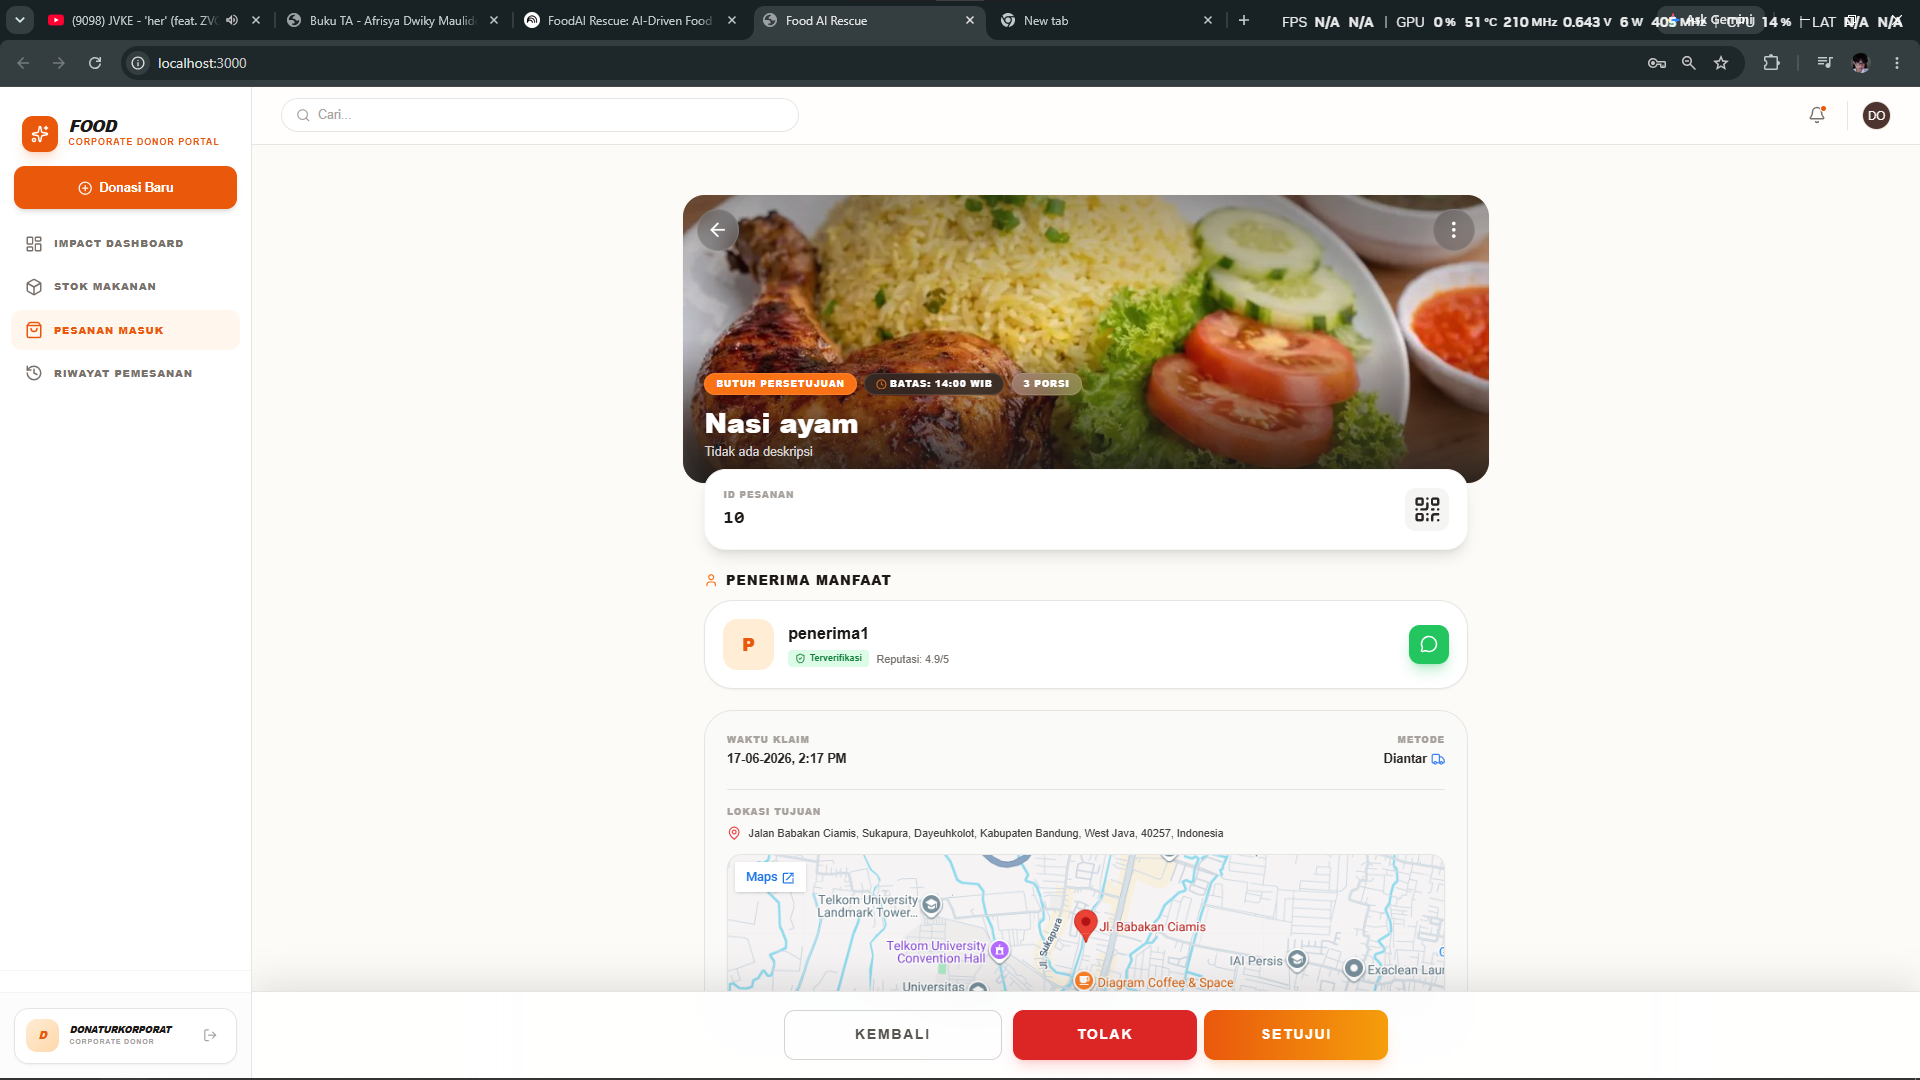
\includegraphics[width=\linewidth]{image/bab4/UserManual/TerimaPesanan/2-DetailRequest.png}
    \caption{Detail Permintaan (\textit{Request})}
\end{figure}



\subsubsection{Proses Verifikasi Penyerahan Donasi ke Kurir}
Langkah-langkah untuk mengonfirmasi serah terima logistik dengan relawan:
\begin{enumerate}[label=\arabic*.]
    \item Buka menu \textbf{Pesanan Aktif} dan pilih pesanan dengan status \textit{Siap Diambil}.
    \item Buka Detail Pesanan, dan pilih opsi pindai Kode QR atau masukkan resi pengantaran manual milik relawan kurir untuk menyerahkan donasi secara nirkontak.
\end{enumerate}

\begin{figure}[H]
    \centering
    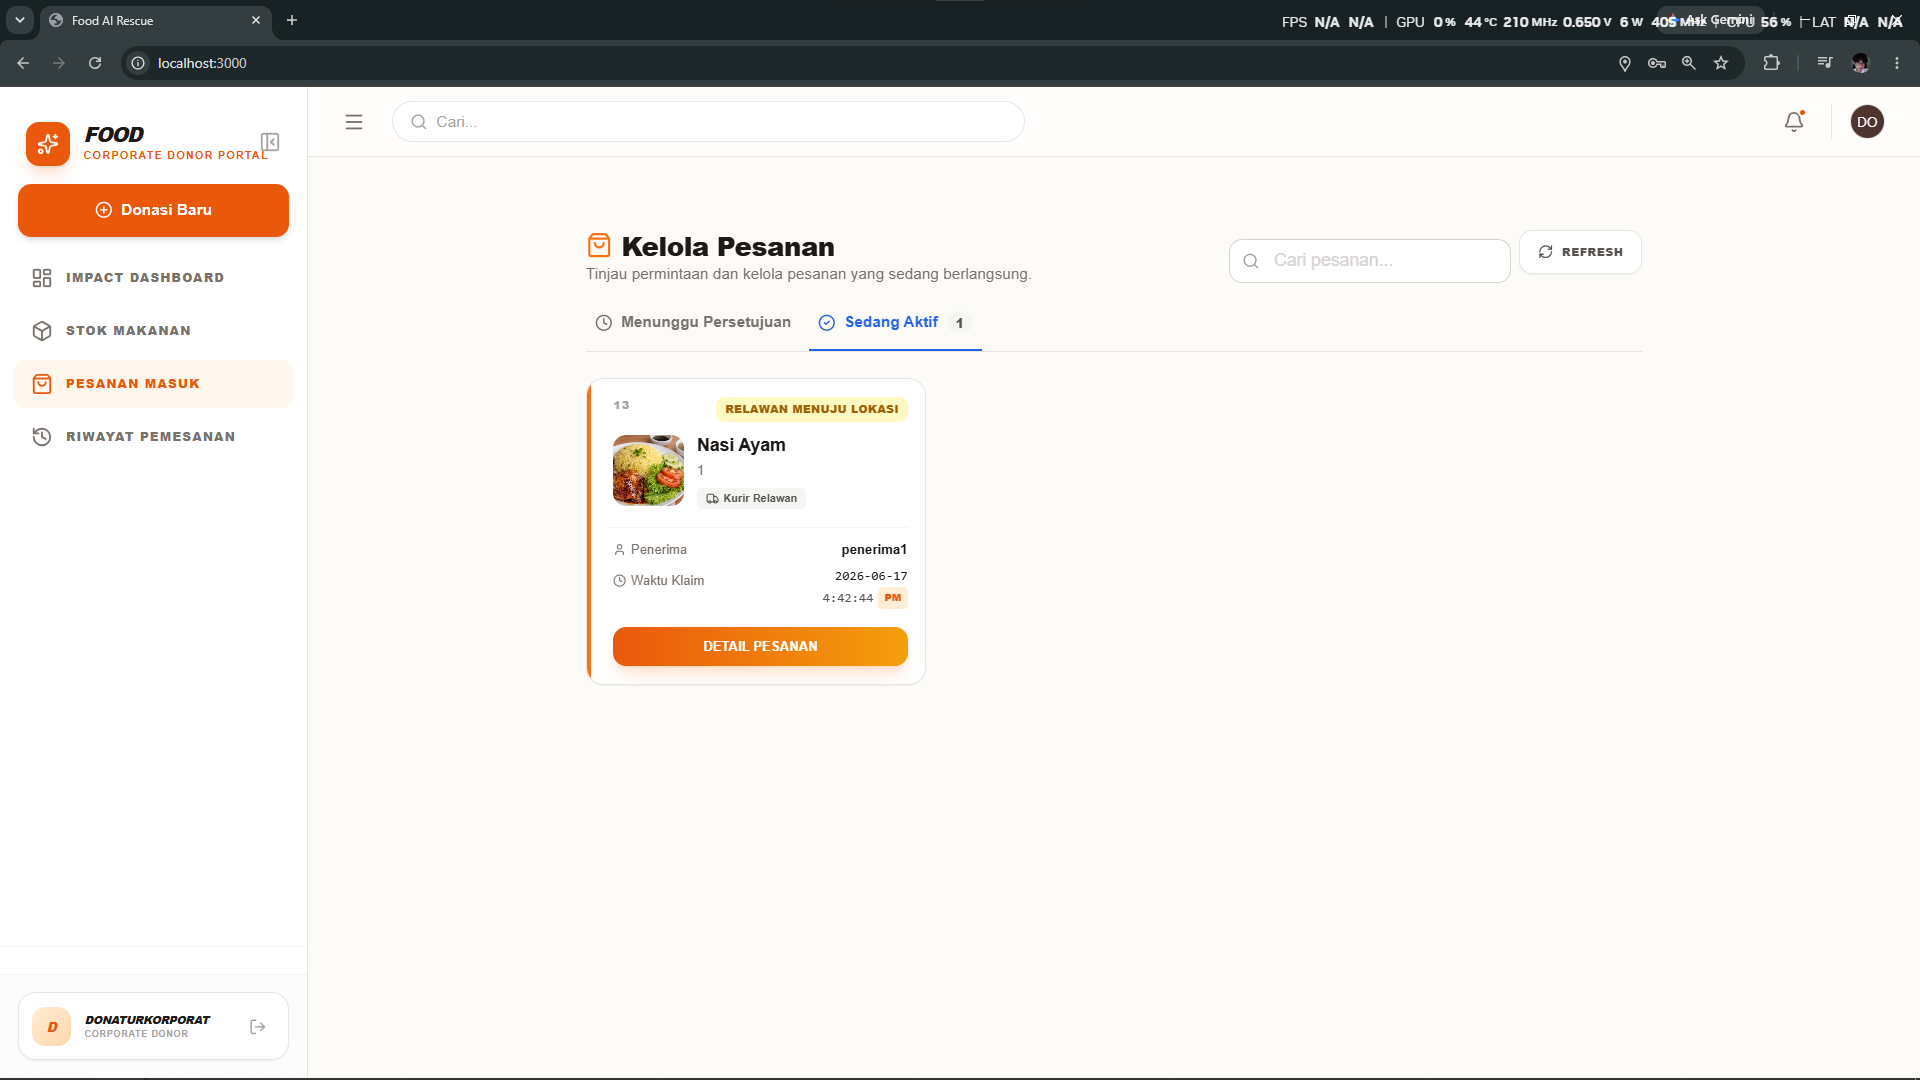
\includegraphics[width=\linewidth]{image/bab4/UserManual/VerifikasiRelawan/1-KelolaPesanan.png}
    \caption{Daftar Pesanan Aktif}
\end{figure}

\begin{figure}[H]
    \centering
    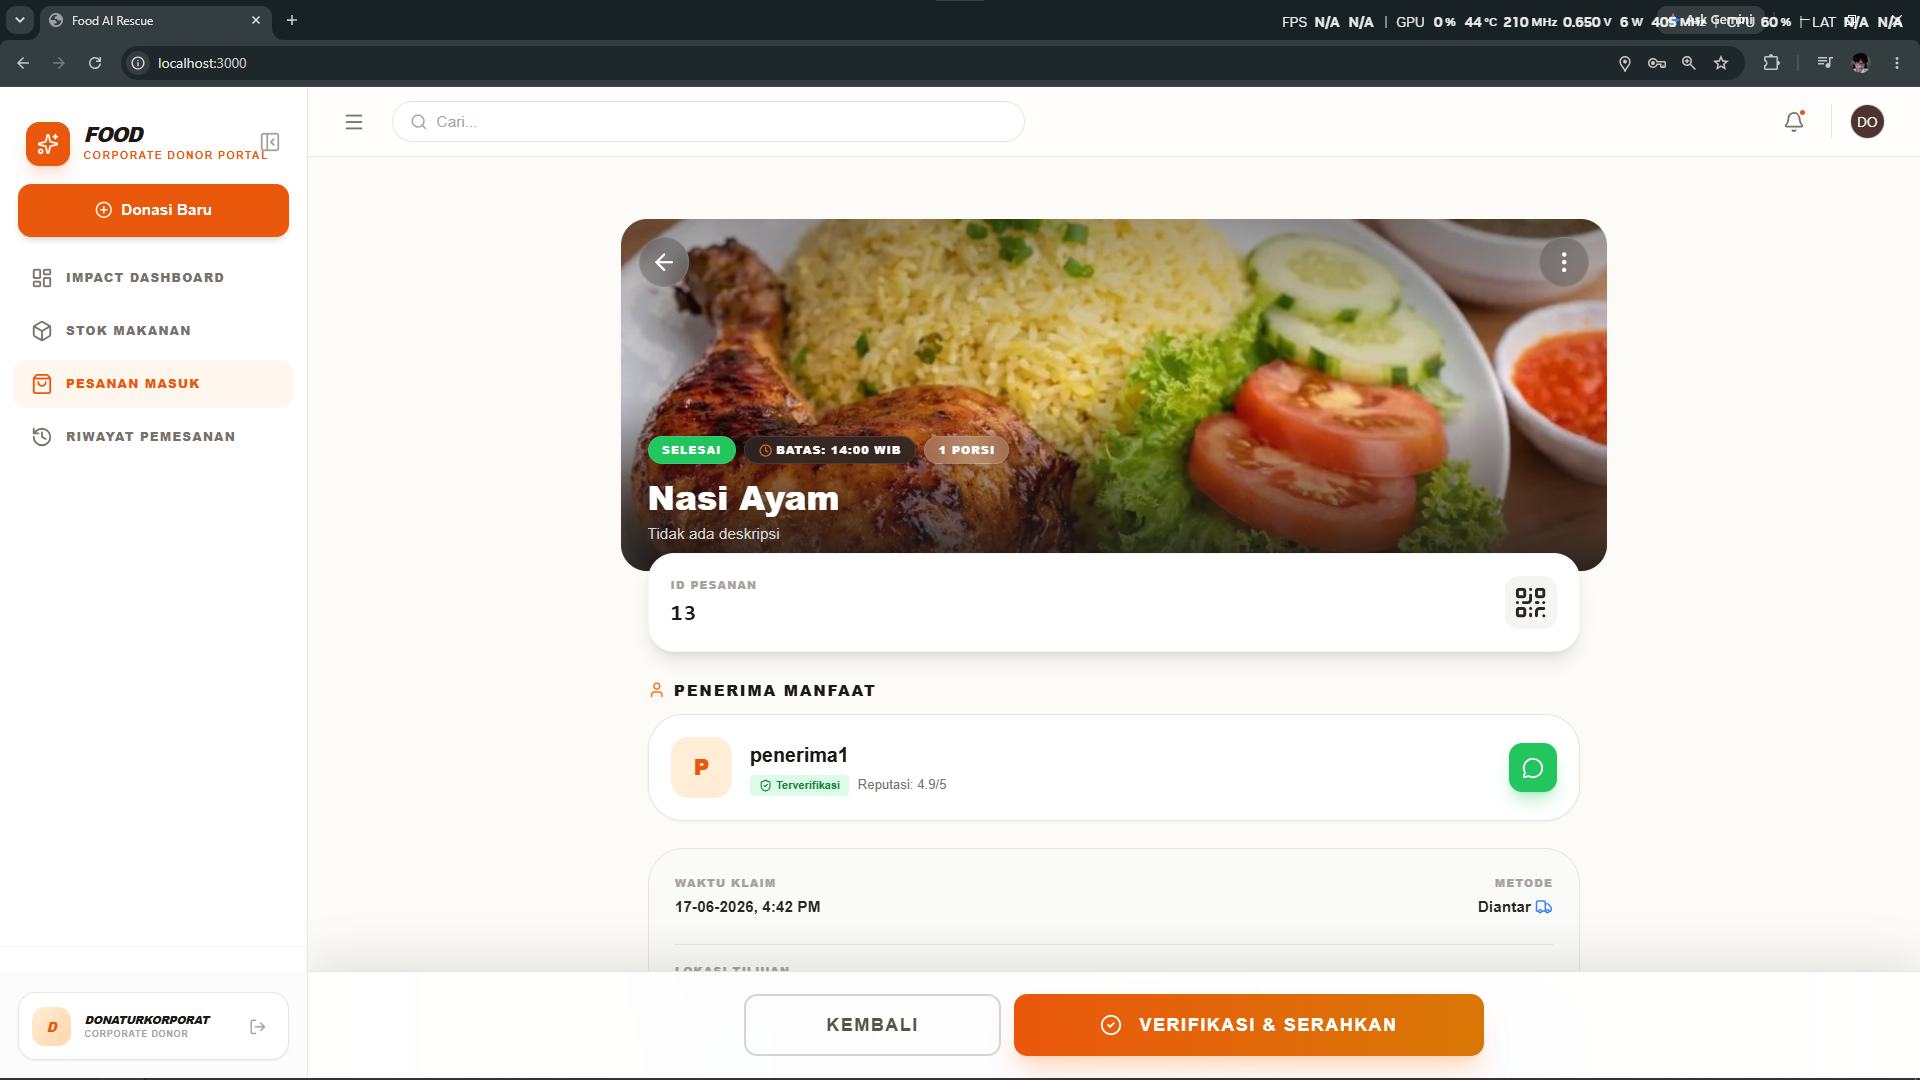
\includegraphics[width=\linewidth]{image/bab4/UserManual/VerifikasiRelawan/2-DetailPesanan.png}
    \caption{Detail Pesanan}
\end{figure}



\begin{figure}[H]
    \centering
    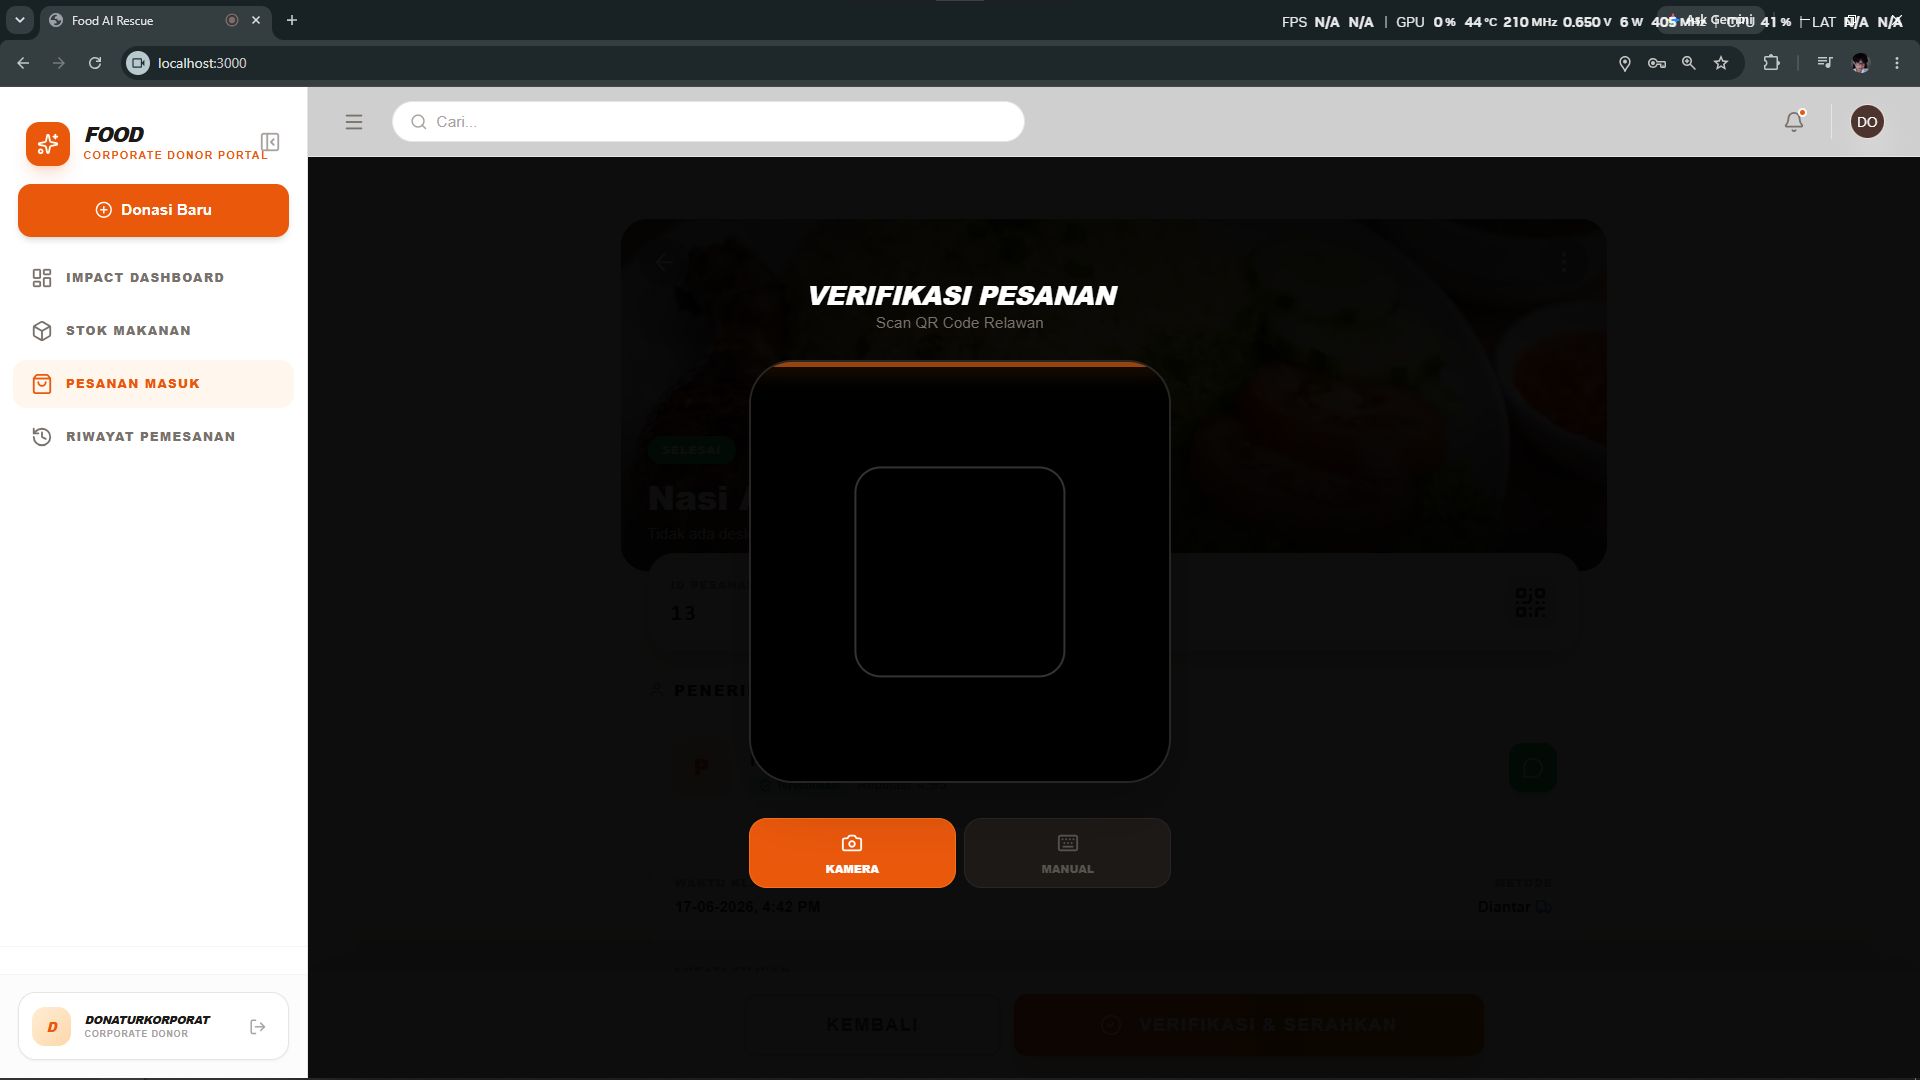
\includegraphics[width=\linewidth]{image/bab4/UserManual/VerifikasiRelawan/3-ScanQR.png}
    \caption{\textit{Scan}}
\end{figure}

\begin{figure}[H]
    \centering
    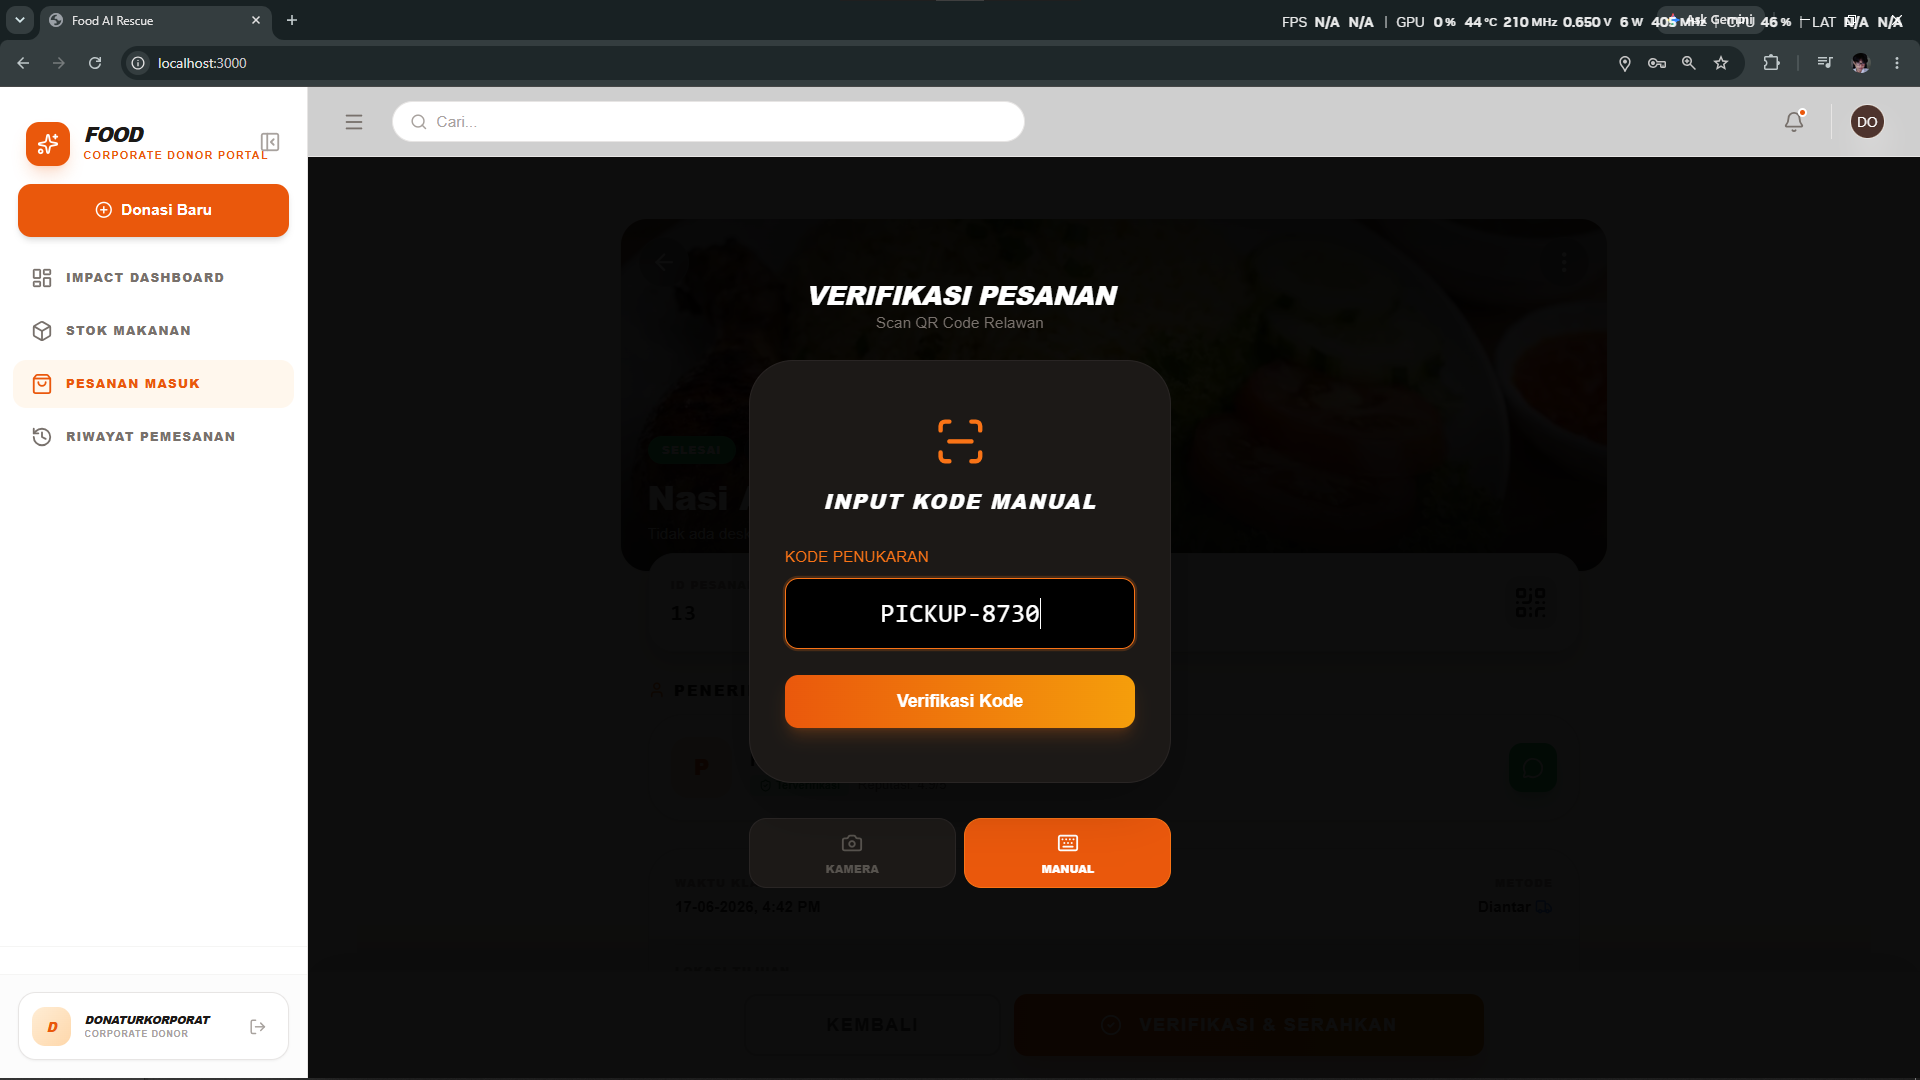
\includegraphics[width=\linewidth]{image/bab4/UserManual/VerifikasiRelawan/4-InputManualCode.png}
    \caption{Input Kode Manual}
\end{figure}



\textbf{C. Pengguna Penerima (Panti Asuhan / Individu)}

\subsubsection{Proses Klaim Donasi Makanan}
Langkah-langkah untuk melakukan pemesanan (klaim) surplus makanan:
\begin{enumerate}[label=\arabic*.]
    \item Buka dasbor radar penerima (\textit{Home Radar}) untuk menelusuri ketersediaan donasi terdekat.
    \item Tekan pada makanan yang diinginkan untuk membaca detail kandungan gizi dan jarak.
    \item Tekan tombol \textbf{Klaim Sekarang} dan pilih metode pengiriman, kemudian konfirmasi pesanan tersebut.
    \item Sistem akan menampilkan layar pemberitahuan bahwa klaim telah terkirim.
\end{enumerate}

\begin{figure}[H]
    \centering
    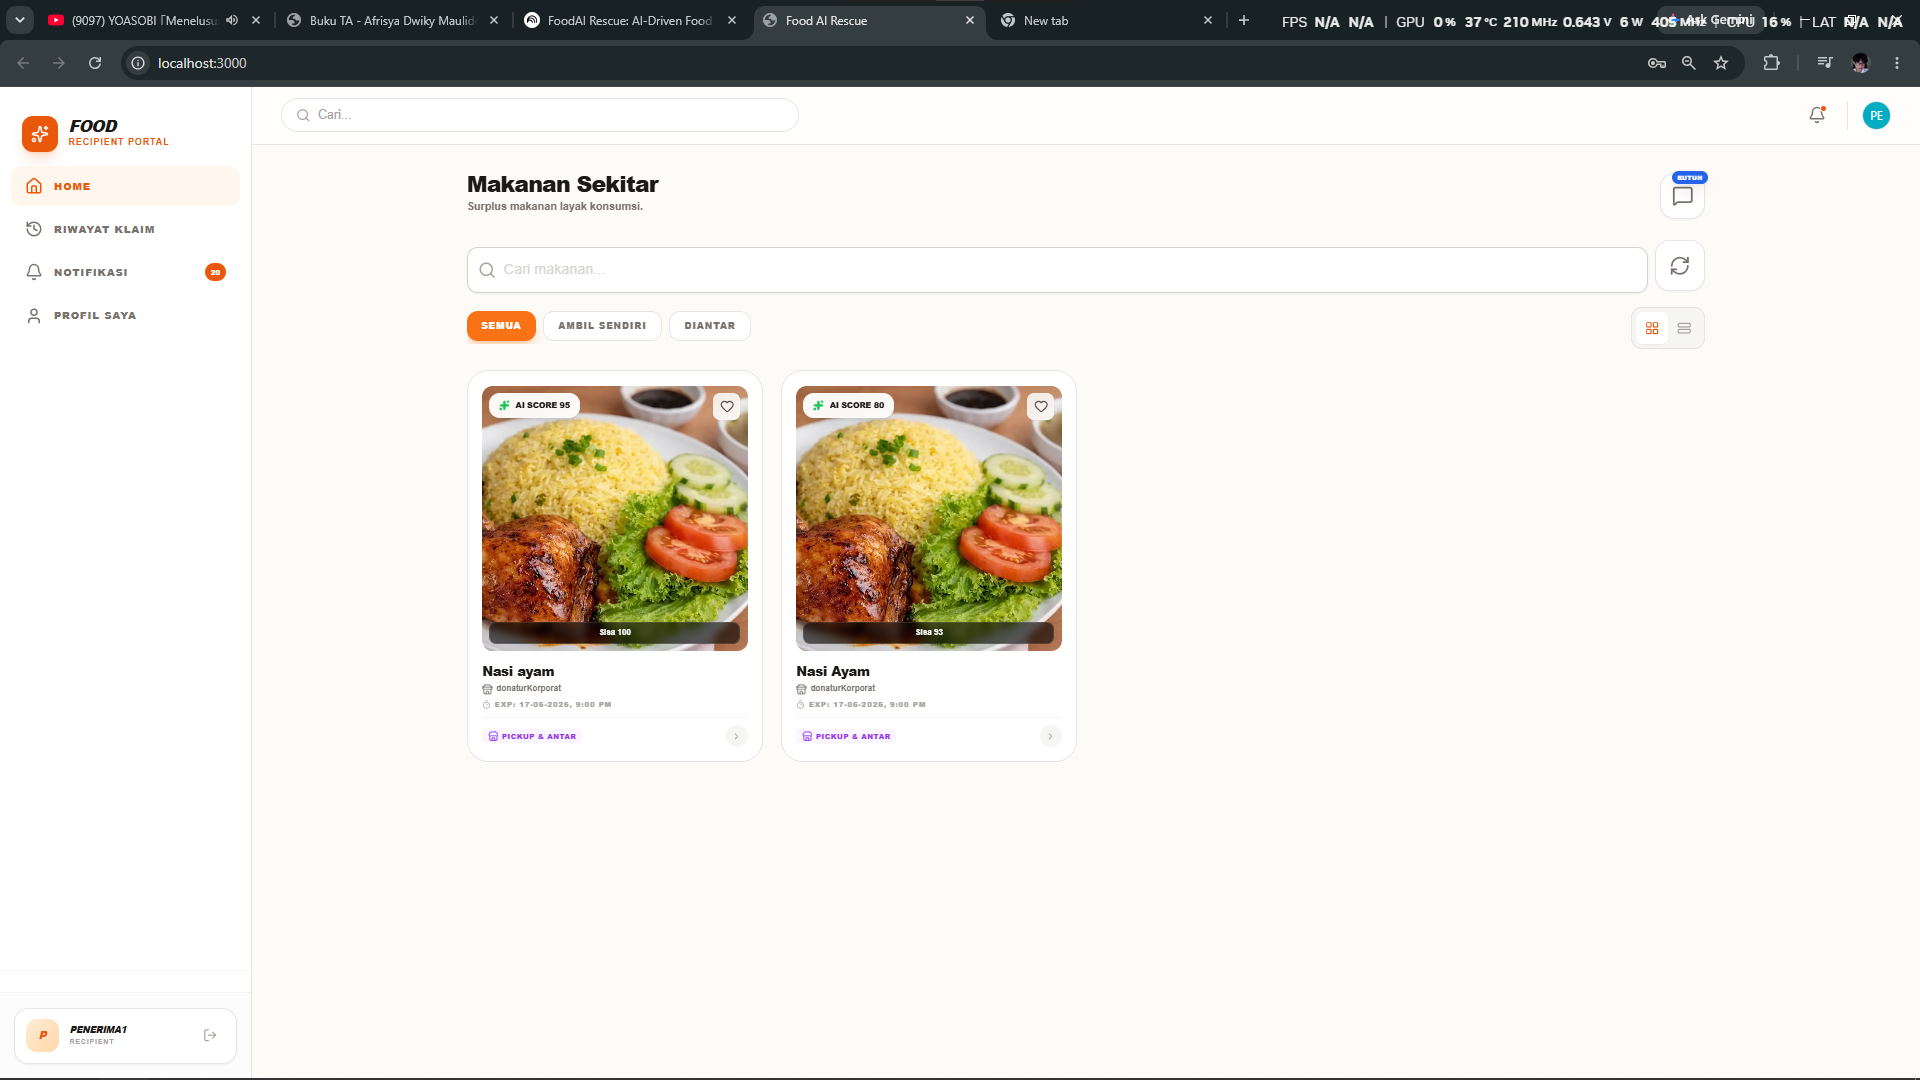
\includegraphics[width=\linewidth]{image/bab4/UserManual/KlaimDonasi/1-HomeRadar.png}
    \caption{Radar Makanan Terdekat}
\end{figure}

\begin{figure}[H]
    \centering
    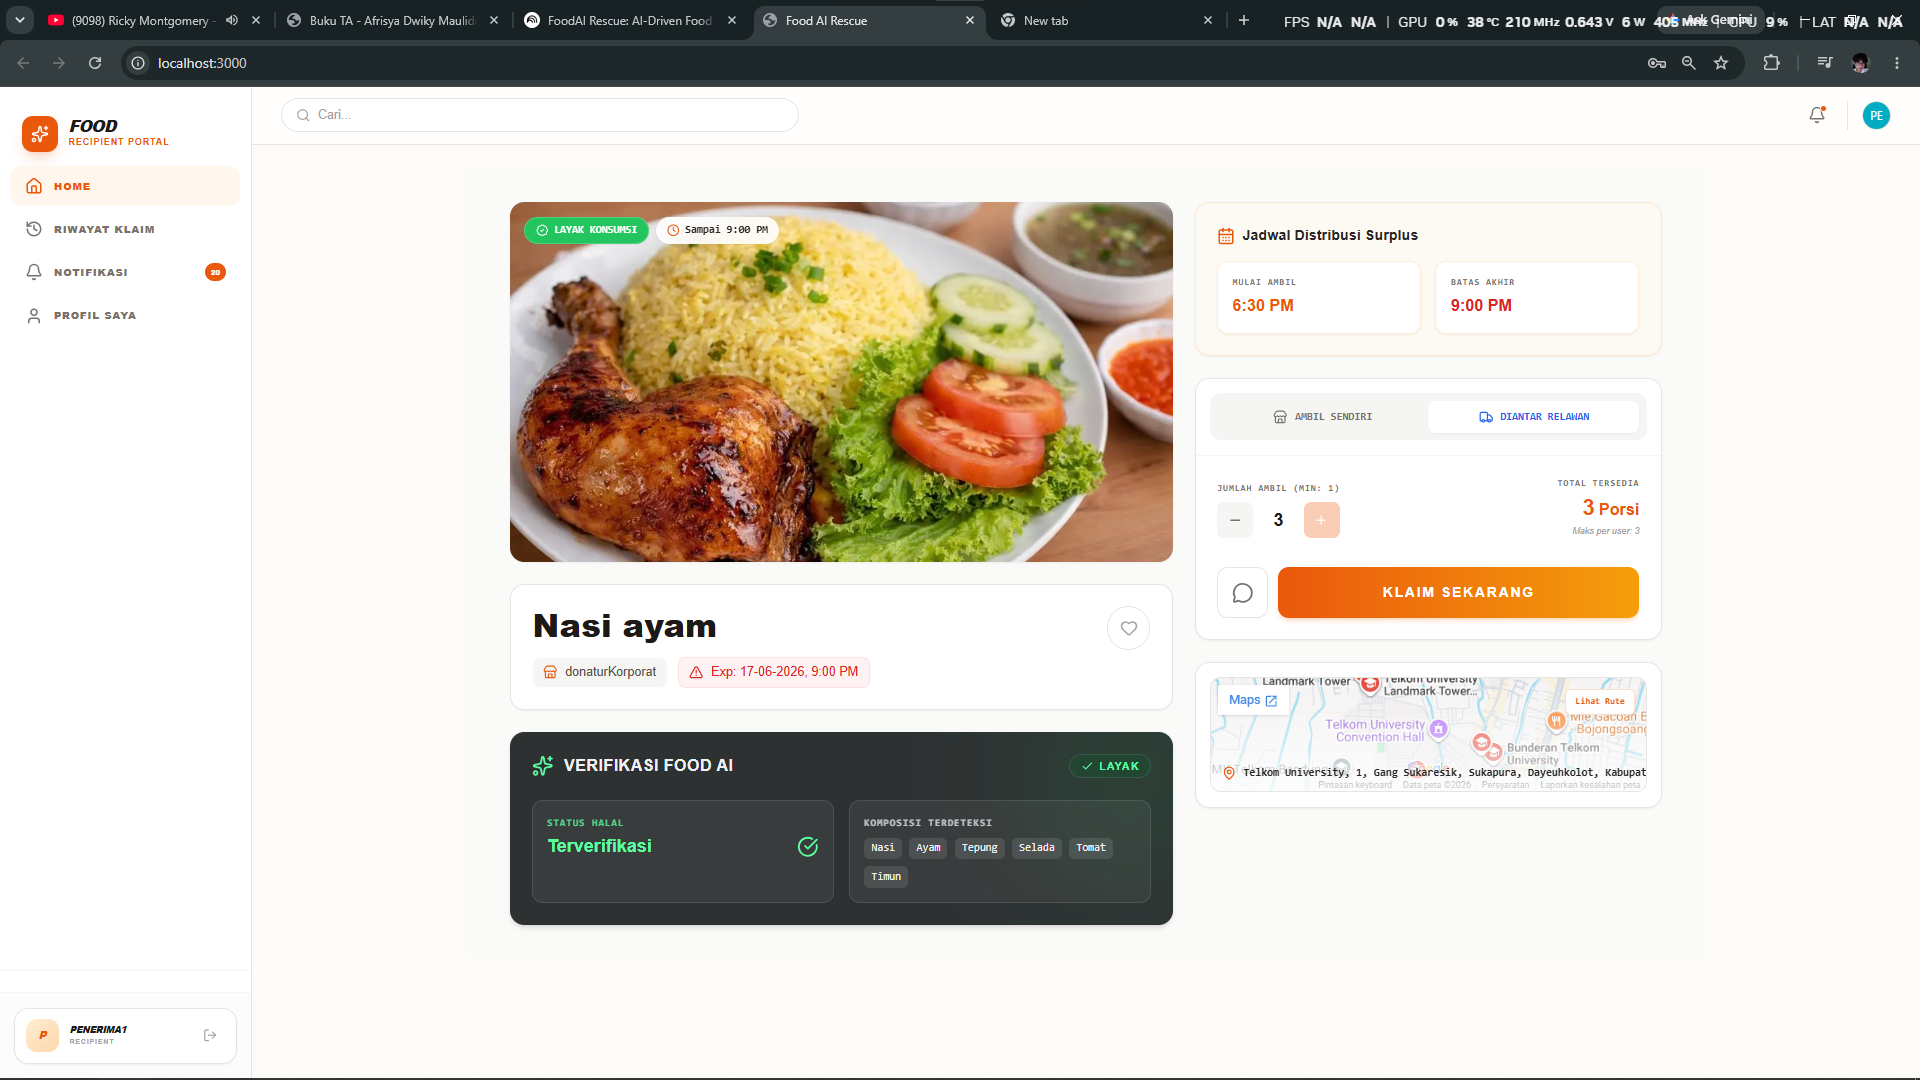
\includegraphics[width=\linewidth]{image/bab4/UserManual/KlaimDonasi/2-DetailMakanan.png}
    \caption{Detail Makanan}
\end{figure}



\begin{figure}[H]
    \centering
    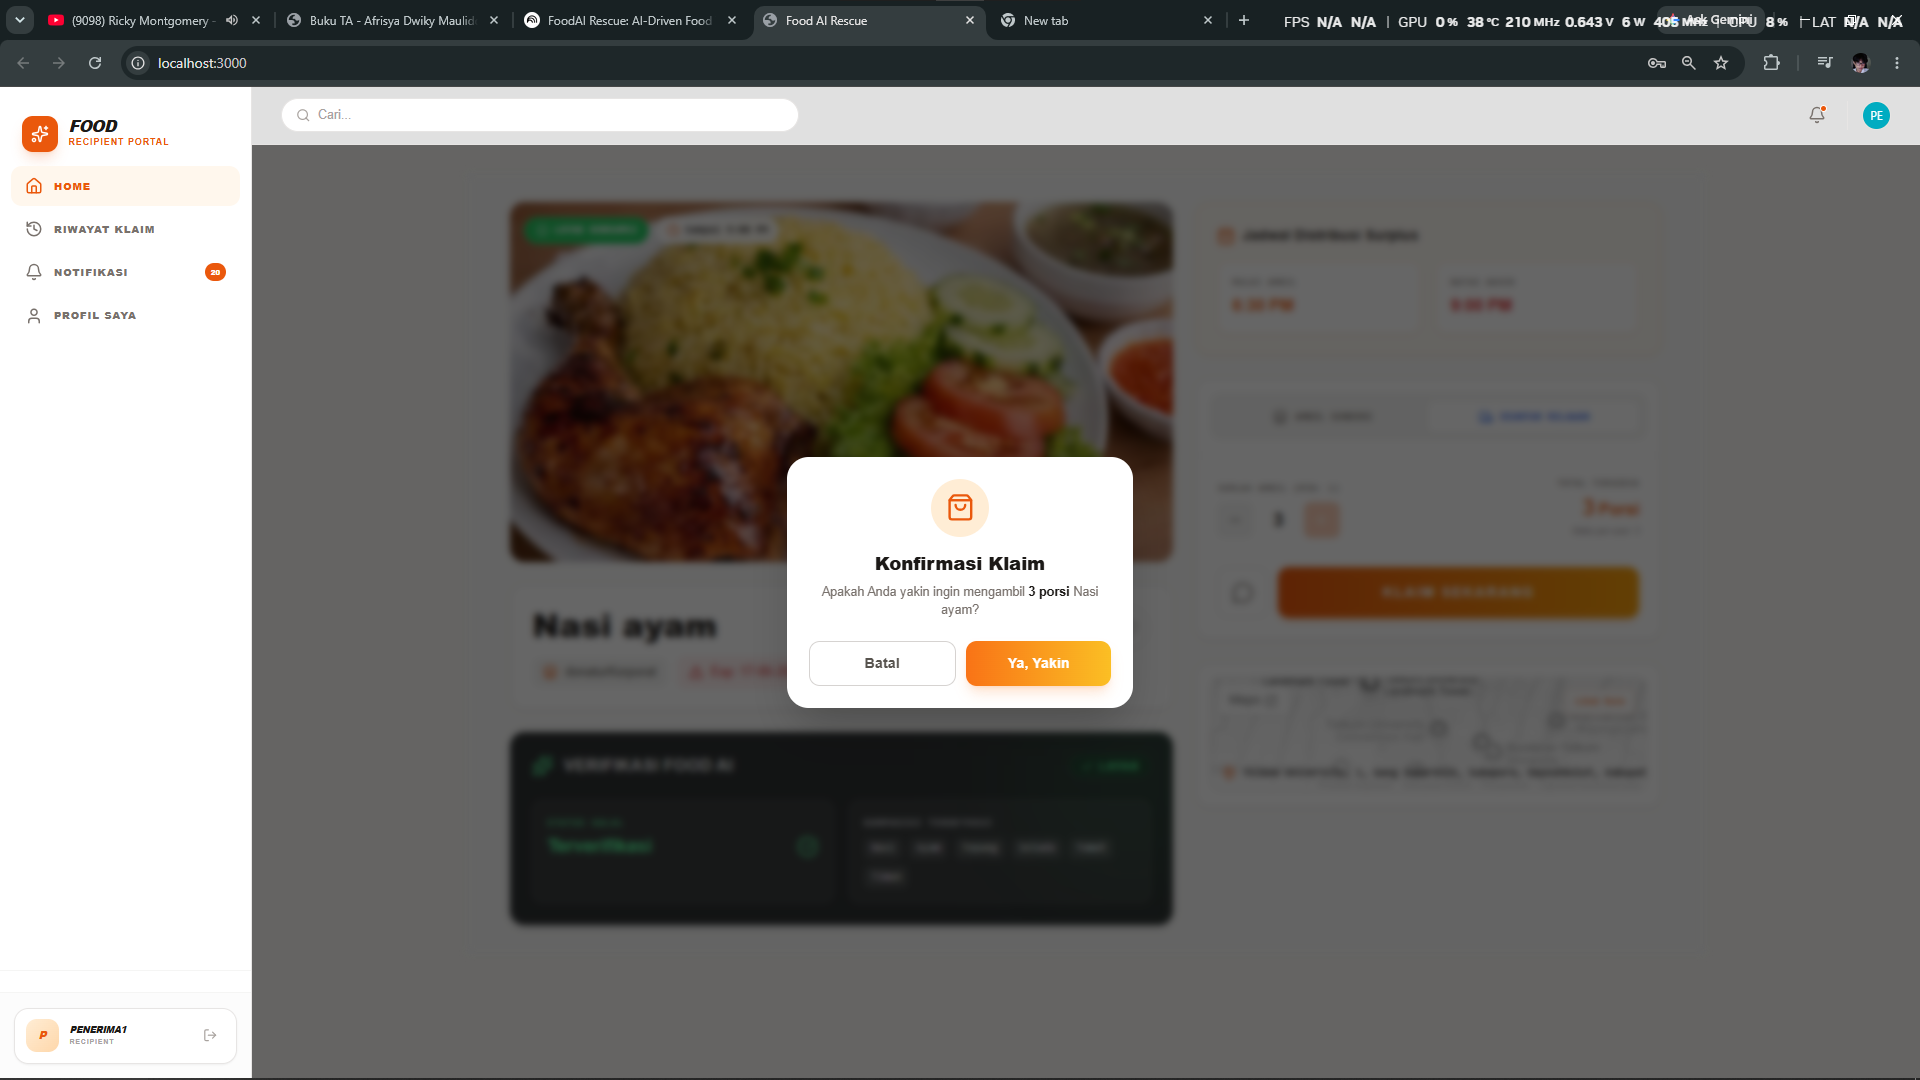
\includegraphics[width=\linewidth]{image/bab4/UserManual/KlaimDonasi/3-KonfirmasiKlaim.png}
    \caption{Konfirmasi Klaim}
\end{figure}

\begin{figure}[H]
    \centering
    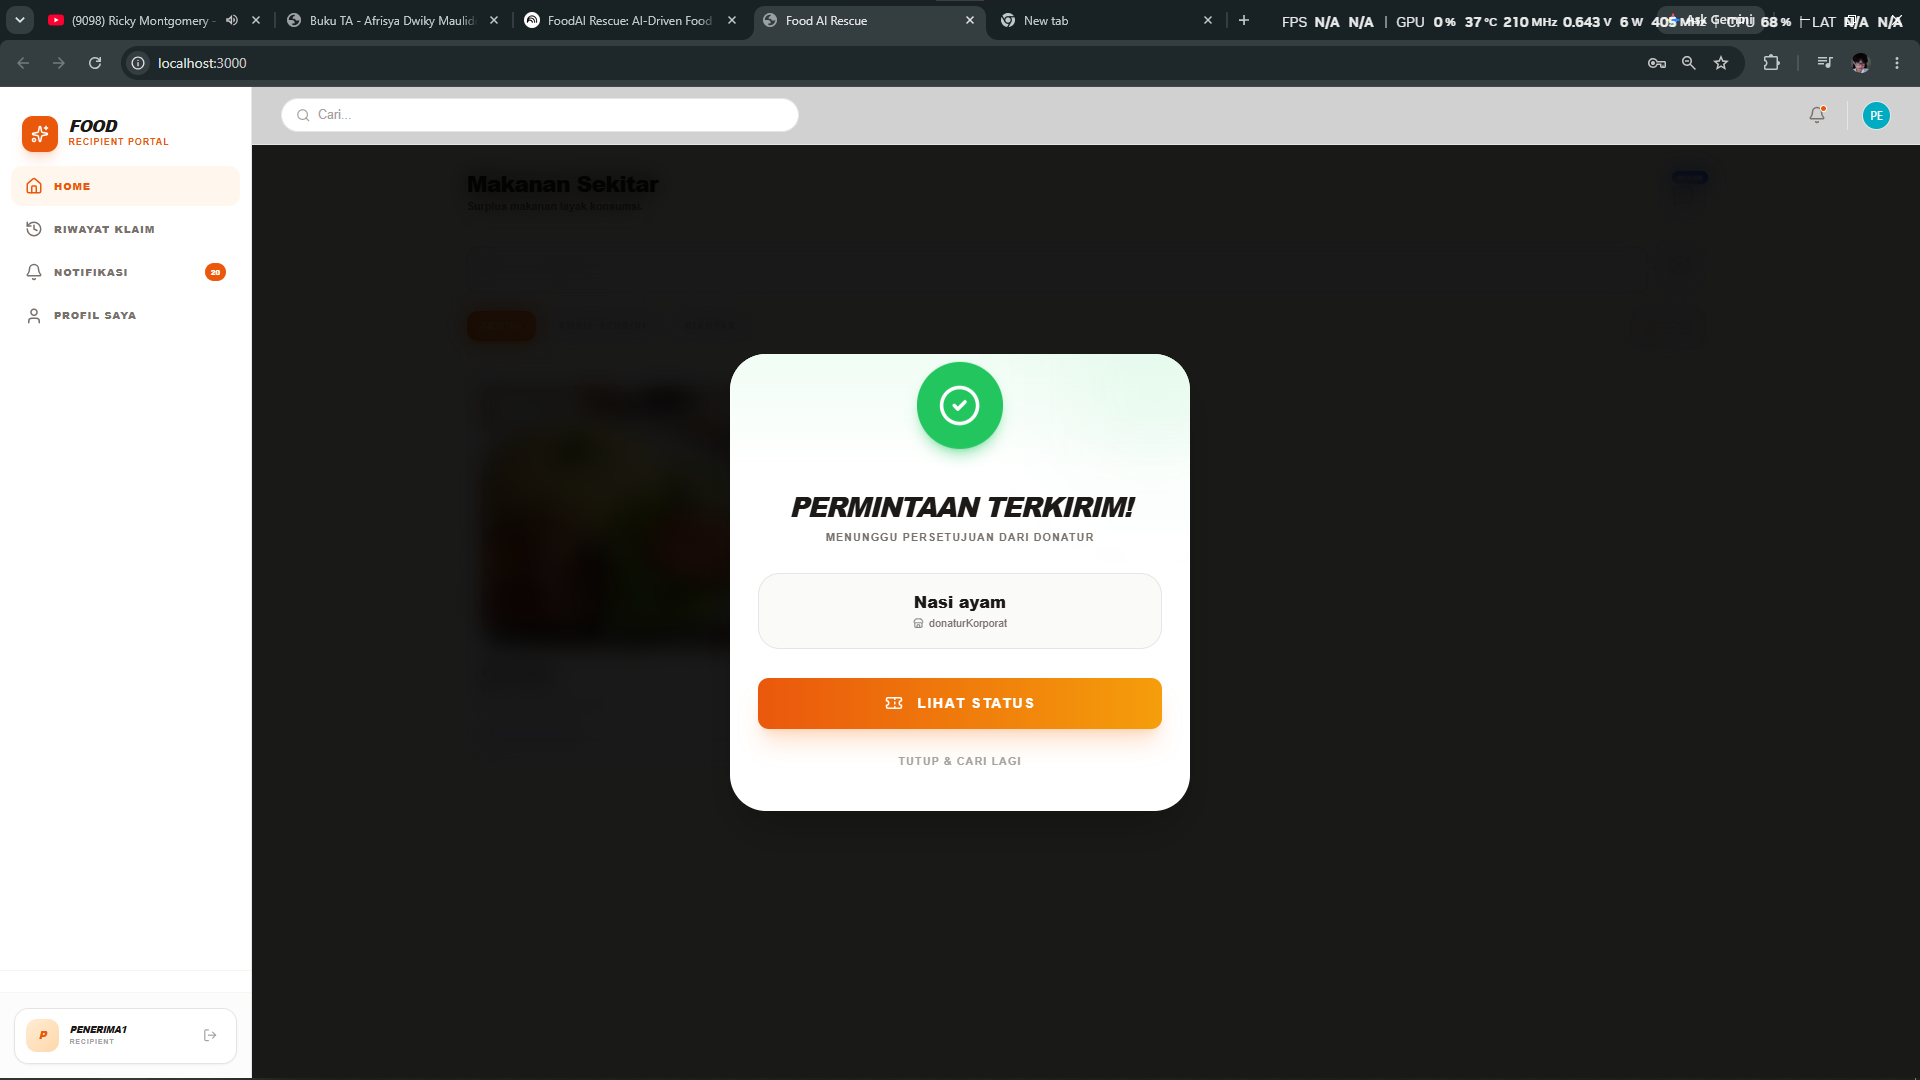
\includegraphics[width=\linewidth]{image/bab4/UserManual/KlaimDonasi/4-KlaimTerkirim.png}
    \caption{Notifikasi Klaim Terkirim}
\end{figure}



\textbf{D. Pengguna Relawan (Kurir Logistik)}

\subsubsection{Proses Mengambil Misi Penjemputan}
Langkah-langkah mengambil misi pengantaran dari katalog tugas:
\begin{enumerate}[label=\arabic*.]
    \item Buka daftar misi antrean pada dasbor \textit{Missions Board}.
    \item Tekan pada salah satu misi untuk melihat manifes rute penjemputan, lalu tekan \textbf{Ambil Misi Ini}.
\end{enumerate}

\begin{figure}[H]
    \centering
    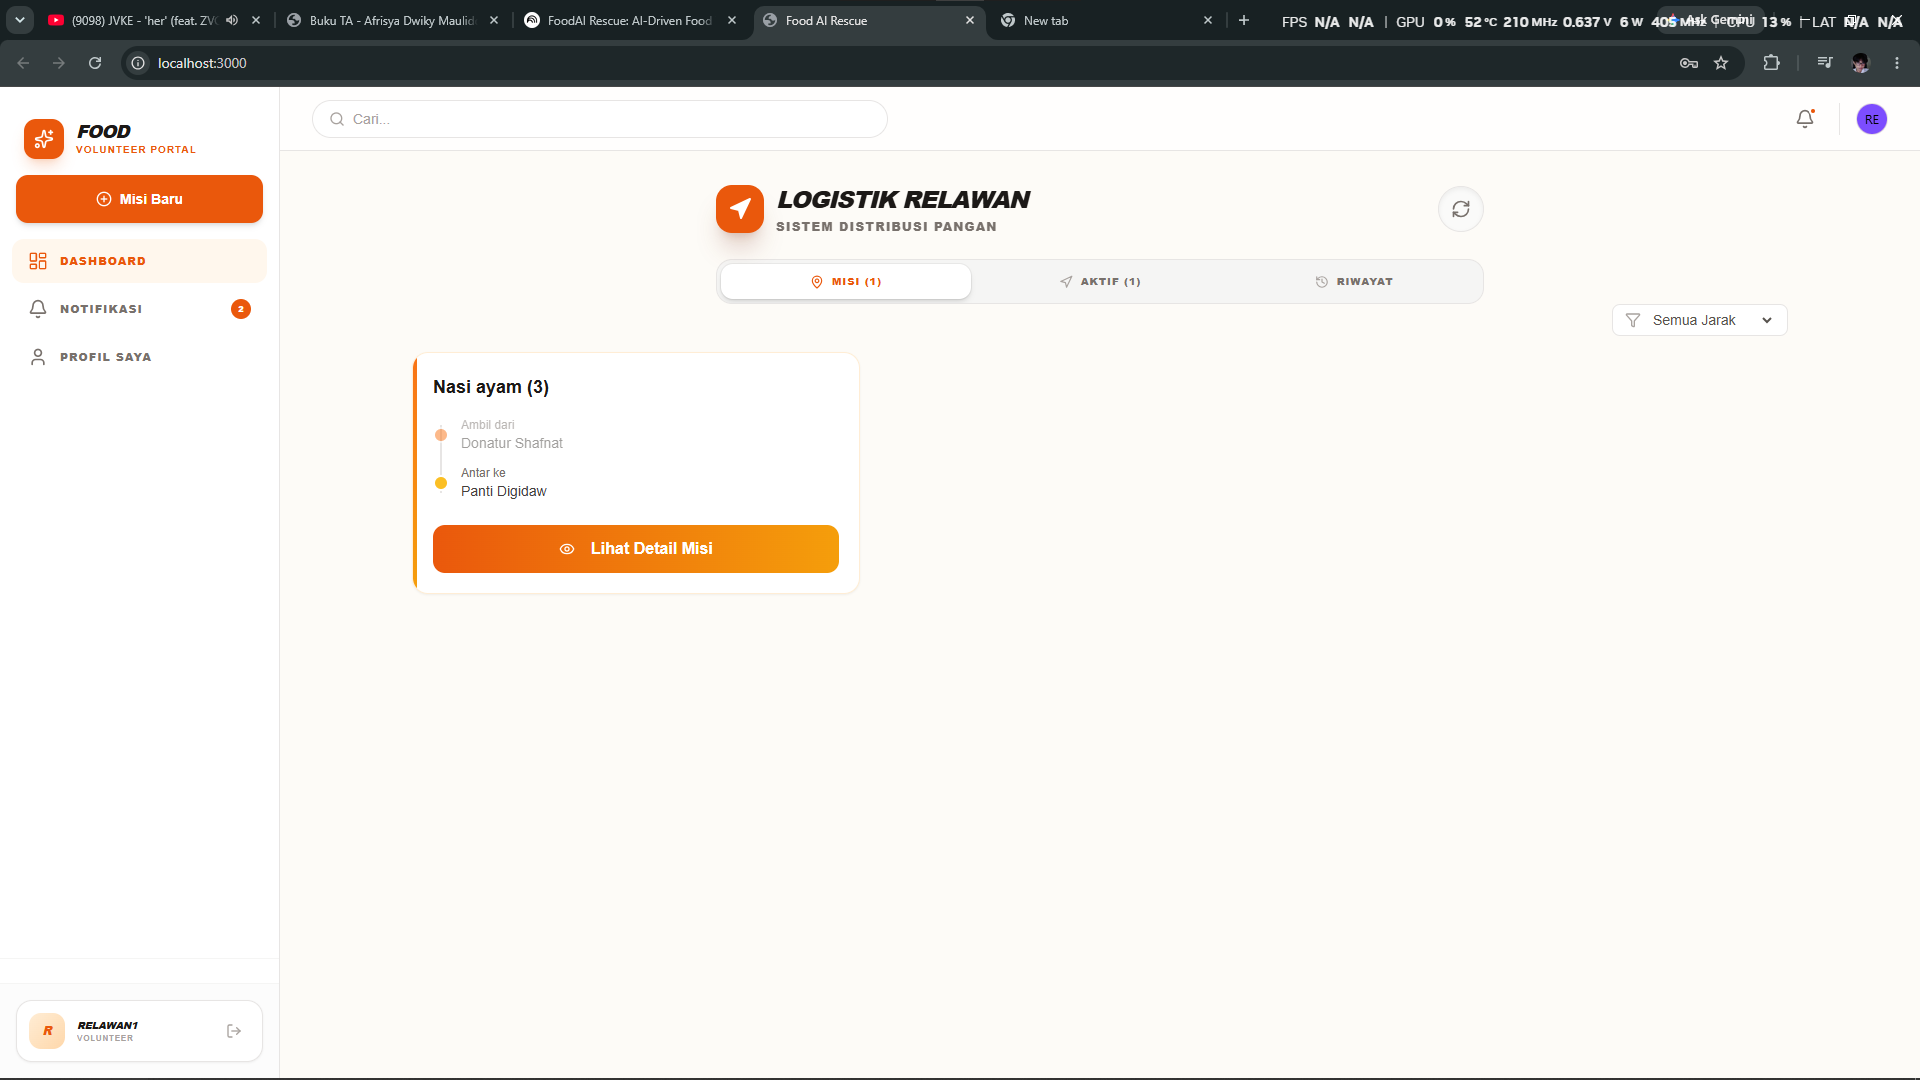
\includegraphics[width=\linewidth]{image/bab4/UserManual/AmbilMisi/1-MissionsBoard.png}
    \caption{Daftar Misi Antrean}
\end{figure}

\begin{figure}[H]
    \centering
    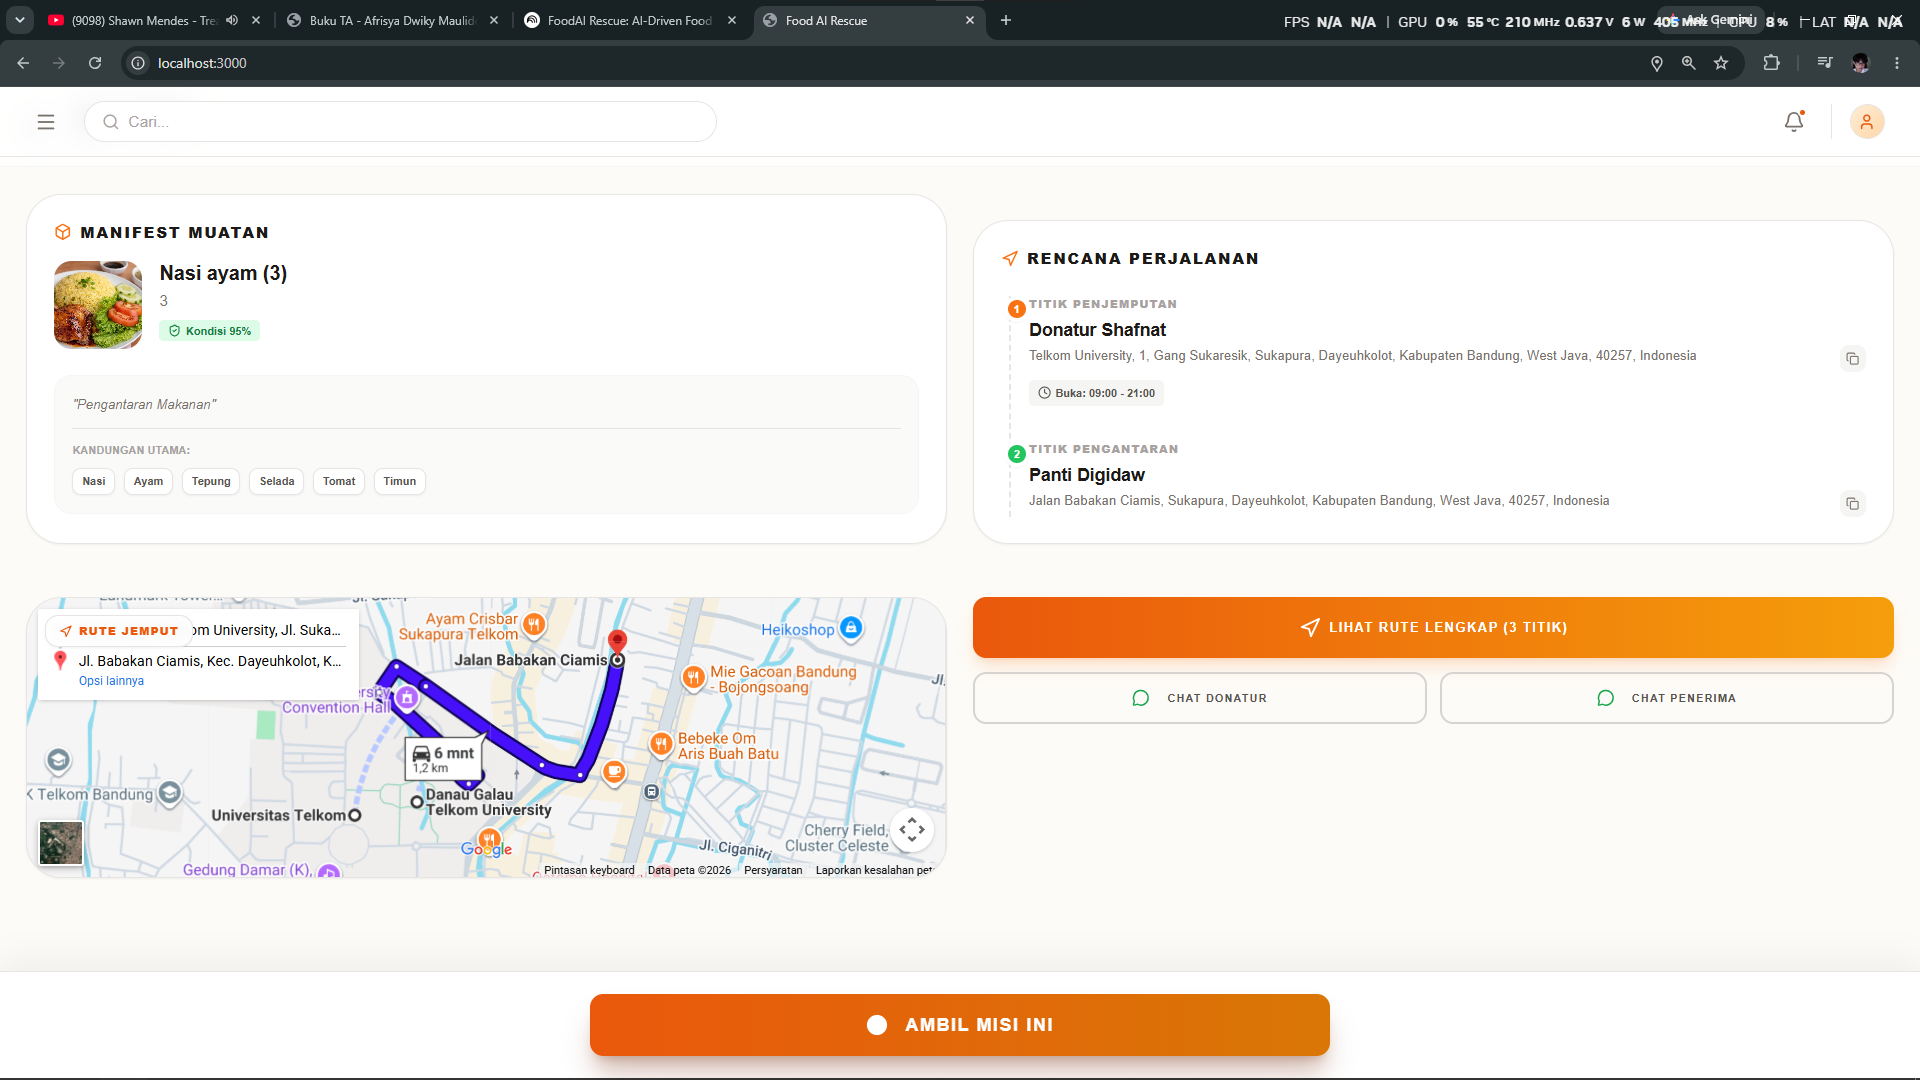
\includegraphics[width=\linewidth]{image/bab4/UserManual/AmbilMisi/2-DetailMisi.png}
    \caption{Detail Penjemputan Misi}
\end{figure}



\subsubsection{Proses Menunjukkan QR Pengambilan Donasi ke Donatur}
Langkah-langkah menunjukkan identitas pengantaran di titik lokasi donatur:
\begin{enumerate}[label=\arabic*.]
    \item Buka daftar \textbf{Misi Aktif} yang sedang berjalan.
    \item Tekan tombol penjemputan untuk memunculkan Kode QR di layar agar dapat dipindai oleh donatur.
\end{enumerate}

\begin{figure}[H]
    \centering
    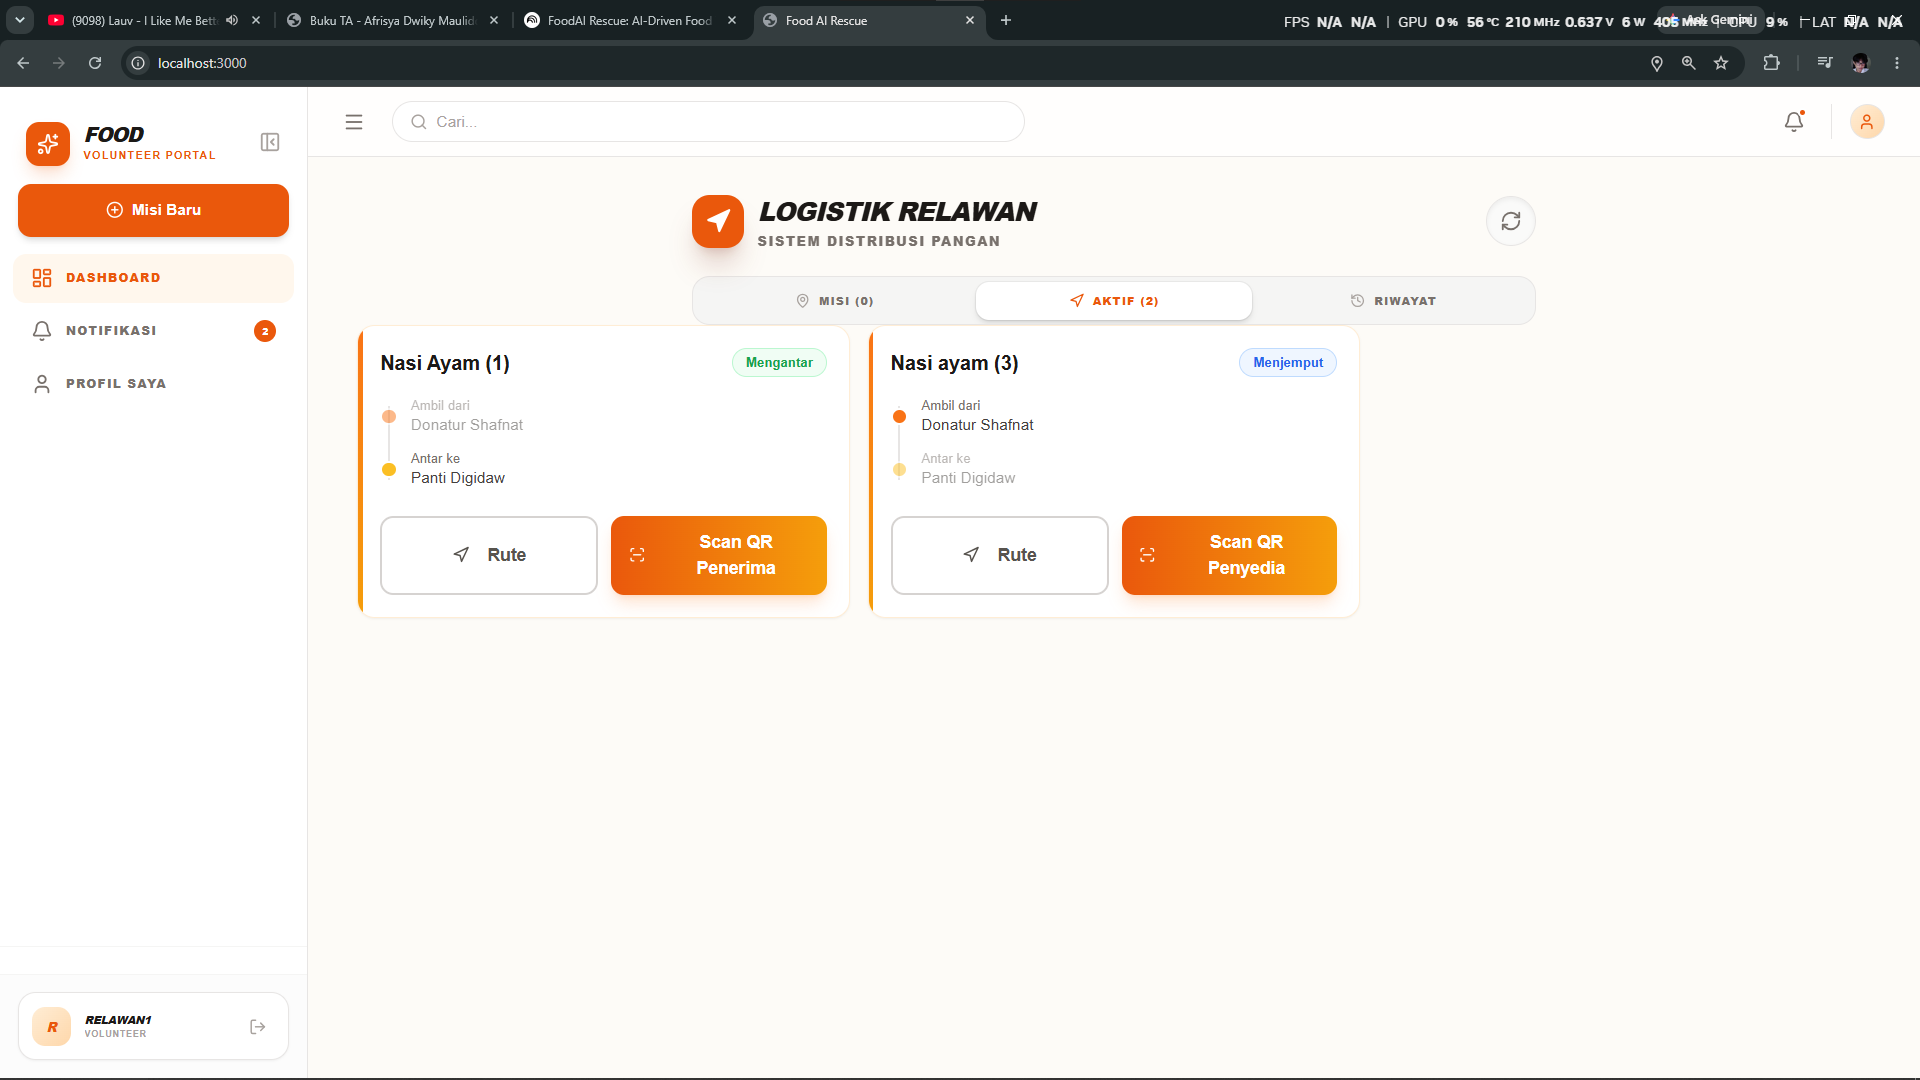
\includegraphics[width=\linewidth]{image/bab4/UserManual/TunjukQR/1-MisiAktif.png}
    \caption{Misi Aktif Logistik}
\end{figure}

\begin{figure}[H]
    \centering
    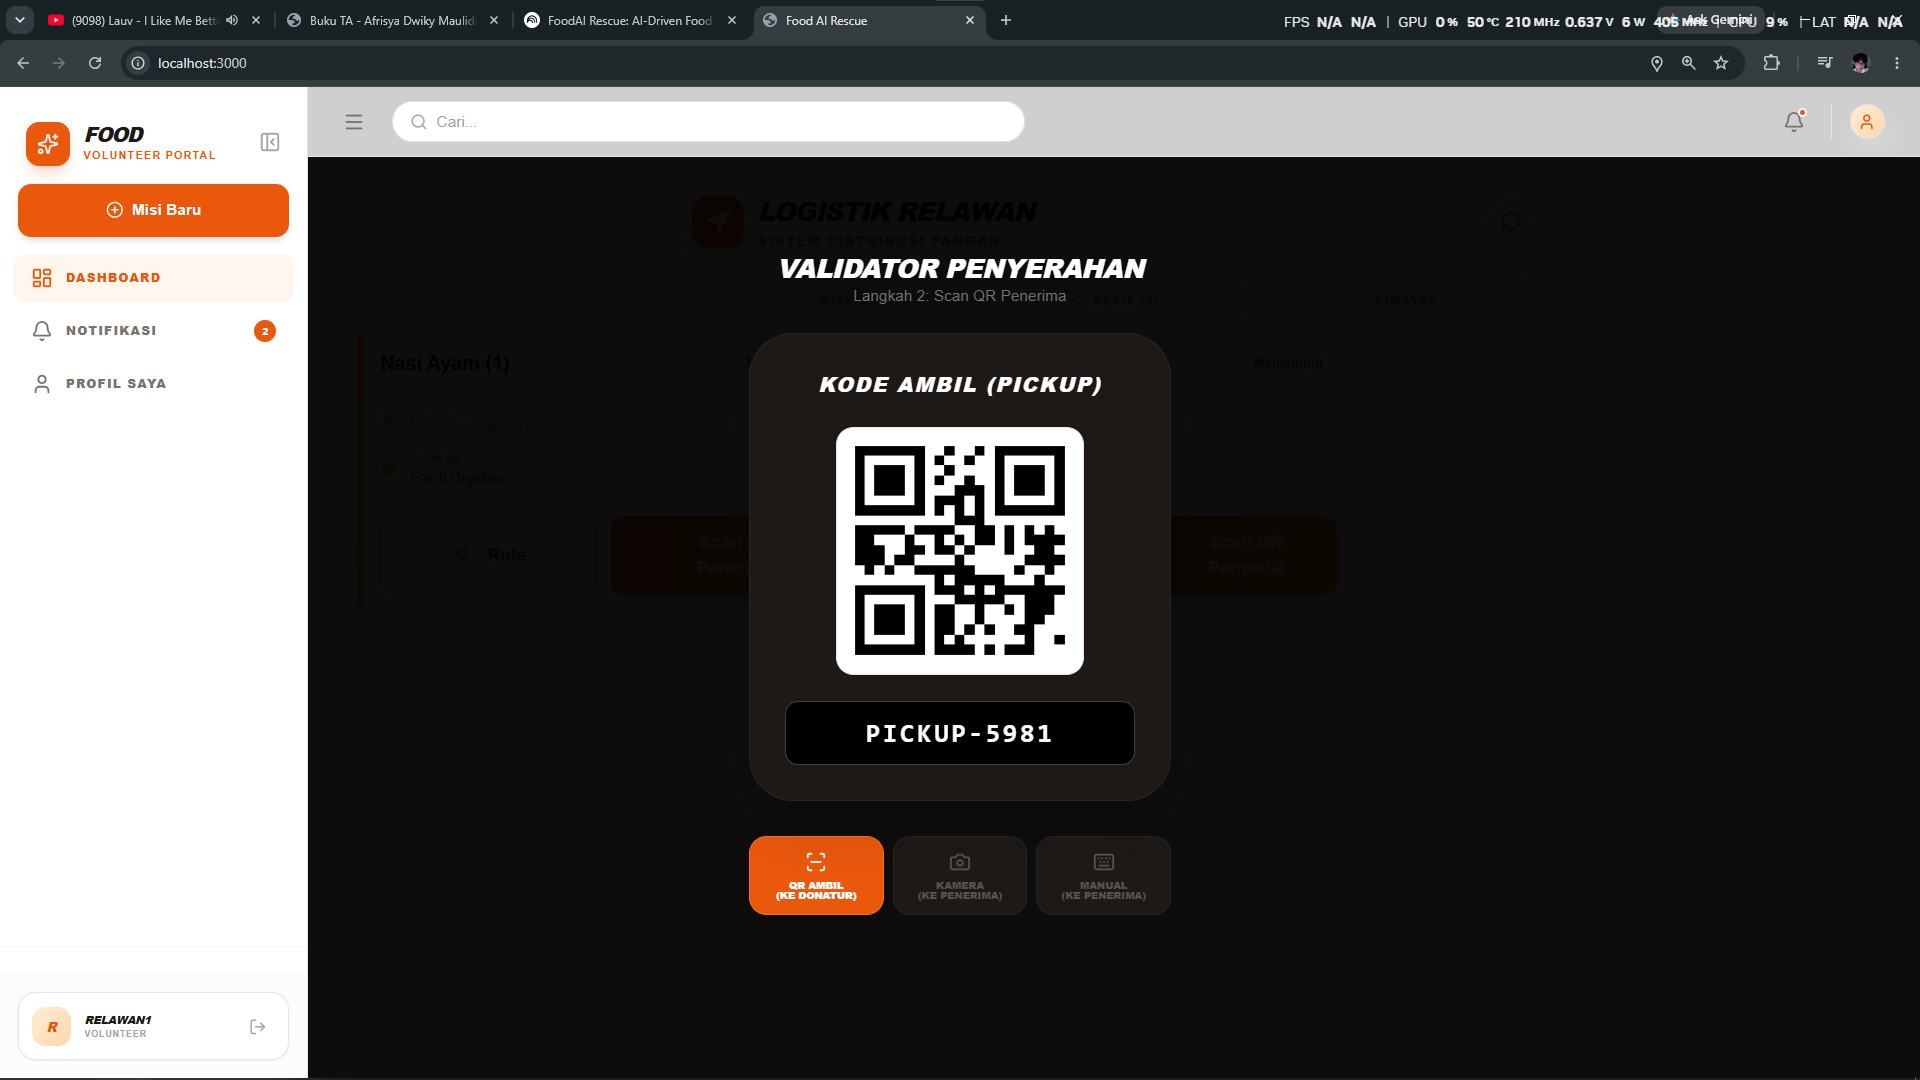
\includegraphics[width=\linewidth]{image/bab4/UserManual/TunjukQR/2-QRPickup.png}
    \caption{\textit{QR Code}}
\end{figure}



\subsubsection{Proses Verifikasi Penyerahan ke Penerima}
Langkah-langkah menyerahkan makanan secara nirkontak di titik tujuan akhir:
\begin{enumerate}[label=\arabic*.]
    \item Saat tiba di alamat penerima, buka kembali layar \textbf{Misi Aktif}.
    \item Tekan tombol verifikasi penerima untuk membuka pemindai kamera (\textit{Scan QR}), atau masukkan kode resi milik penerima melalui opsi \textit{Input Manual}.
\end{enumerate}

\begin{figure}[H]
    \centering
    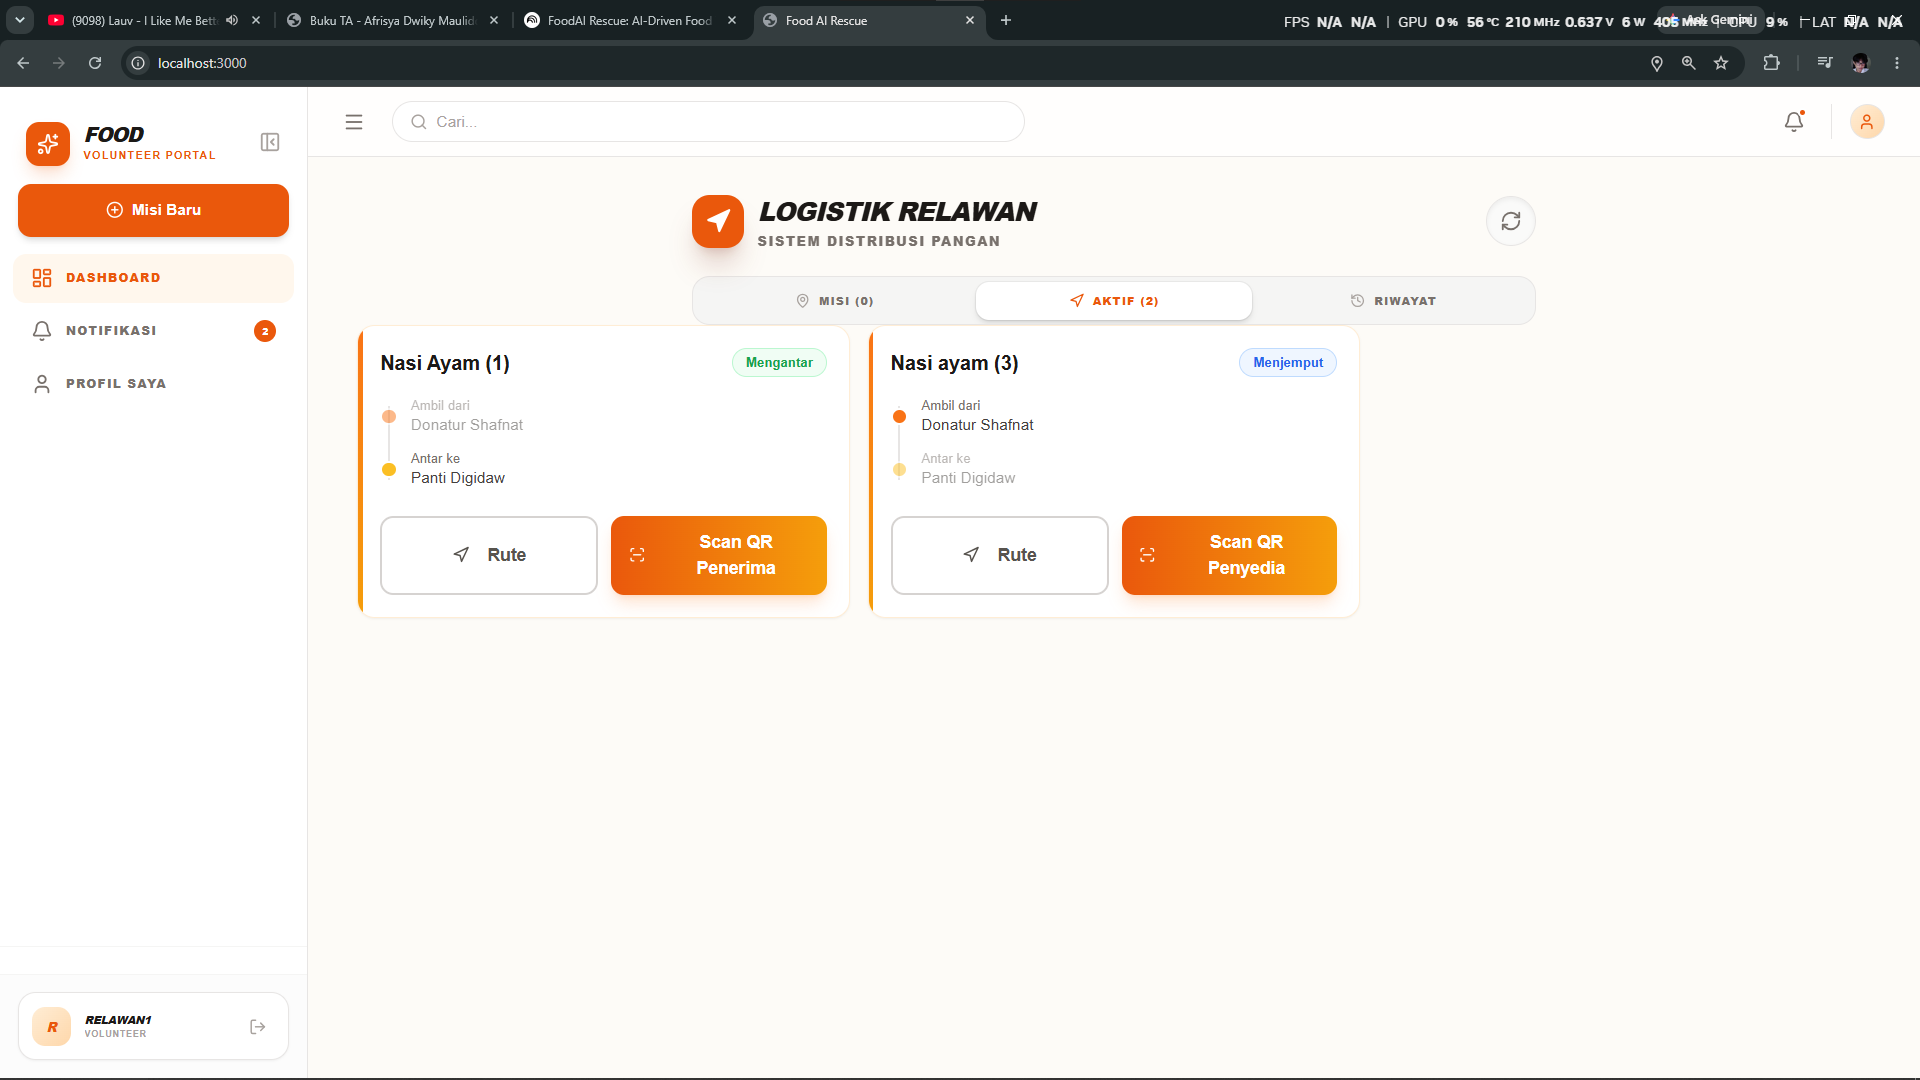
\includegraphics[width=\linewidth]{image/bab4/UserManual/VerifikasiPenerima/1-MisiAktifPengantaran.png}
    \caption{Misi Pengantaran Aktif}
\end{figure}

\begin{figure}[H]
    \centering
    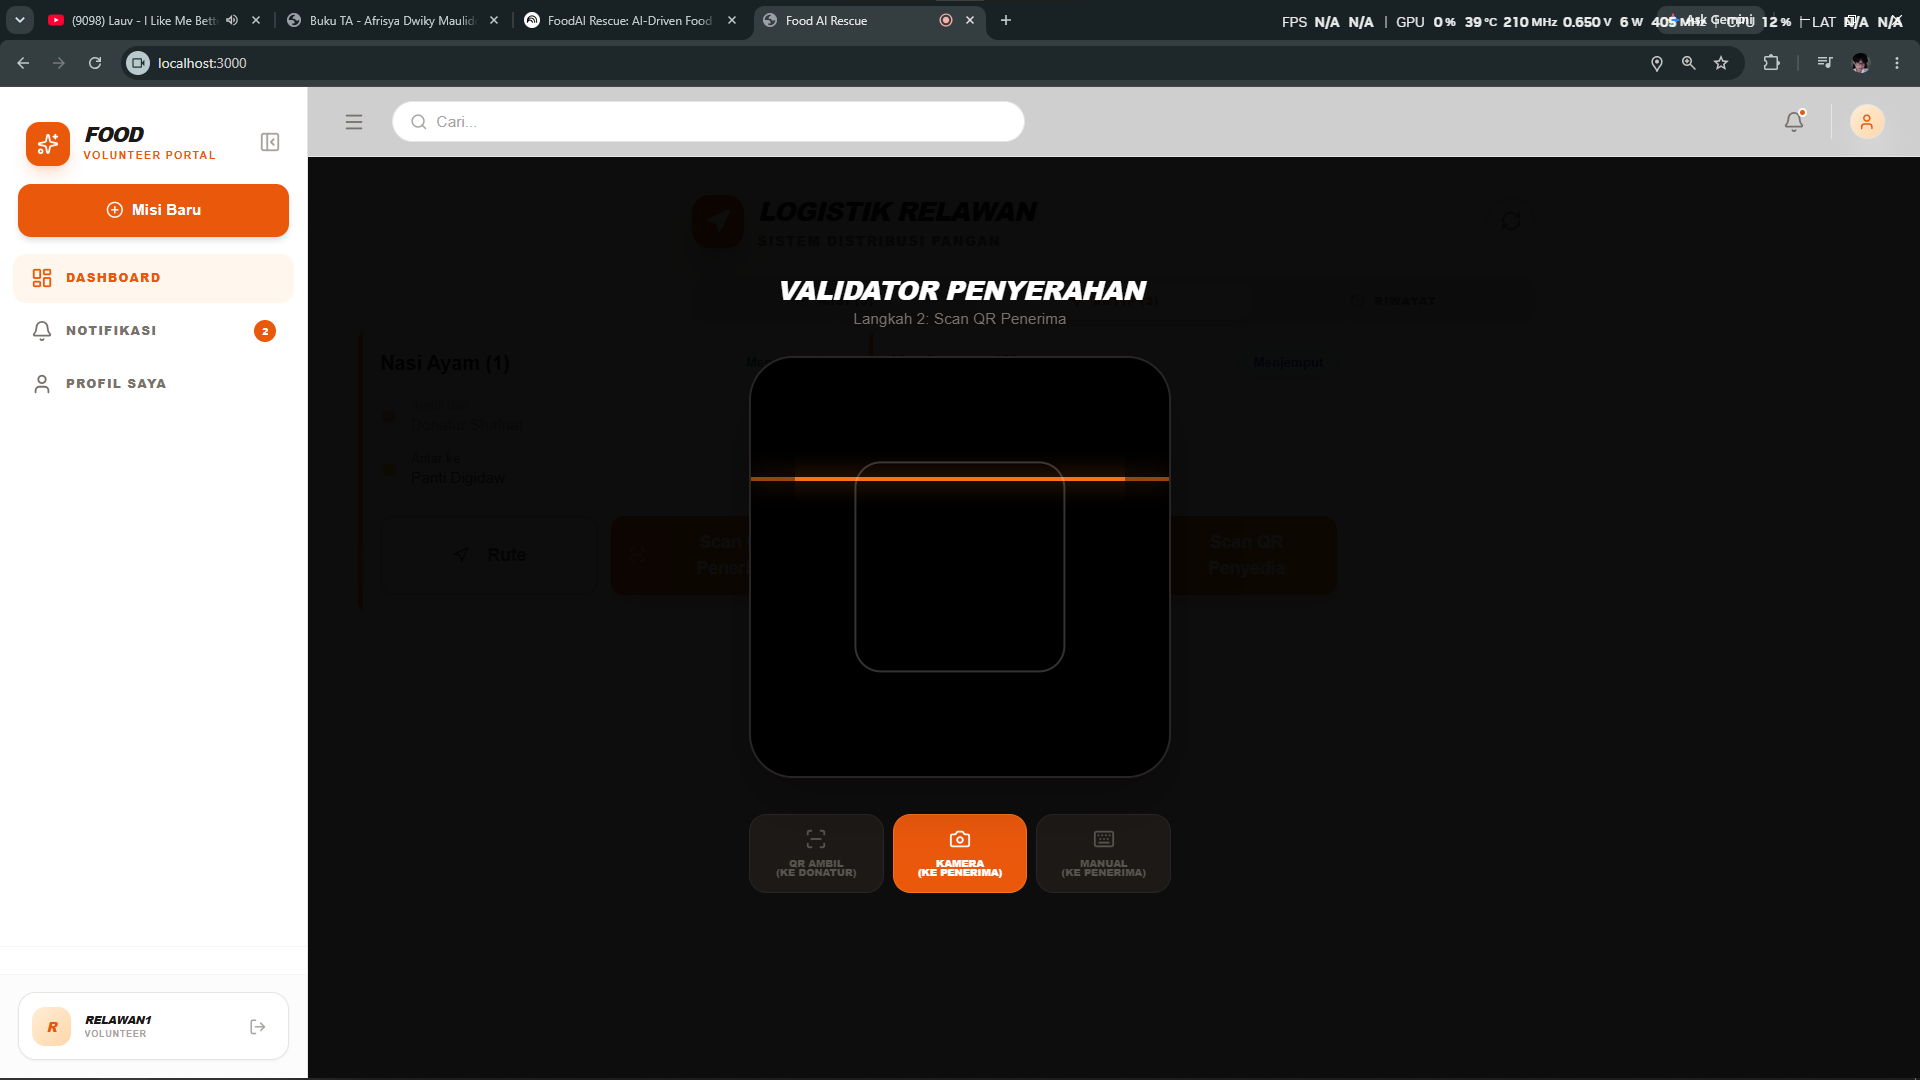
\includegraphics[width=\linewidth]{image/bab4/UserManual/VerifikasiPenerima/3-ScanQR.png}
    \caption{Memindai QR Penerima}
\end{figure}

\begin{figure}[H]
    \centering
    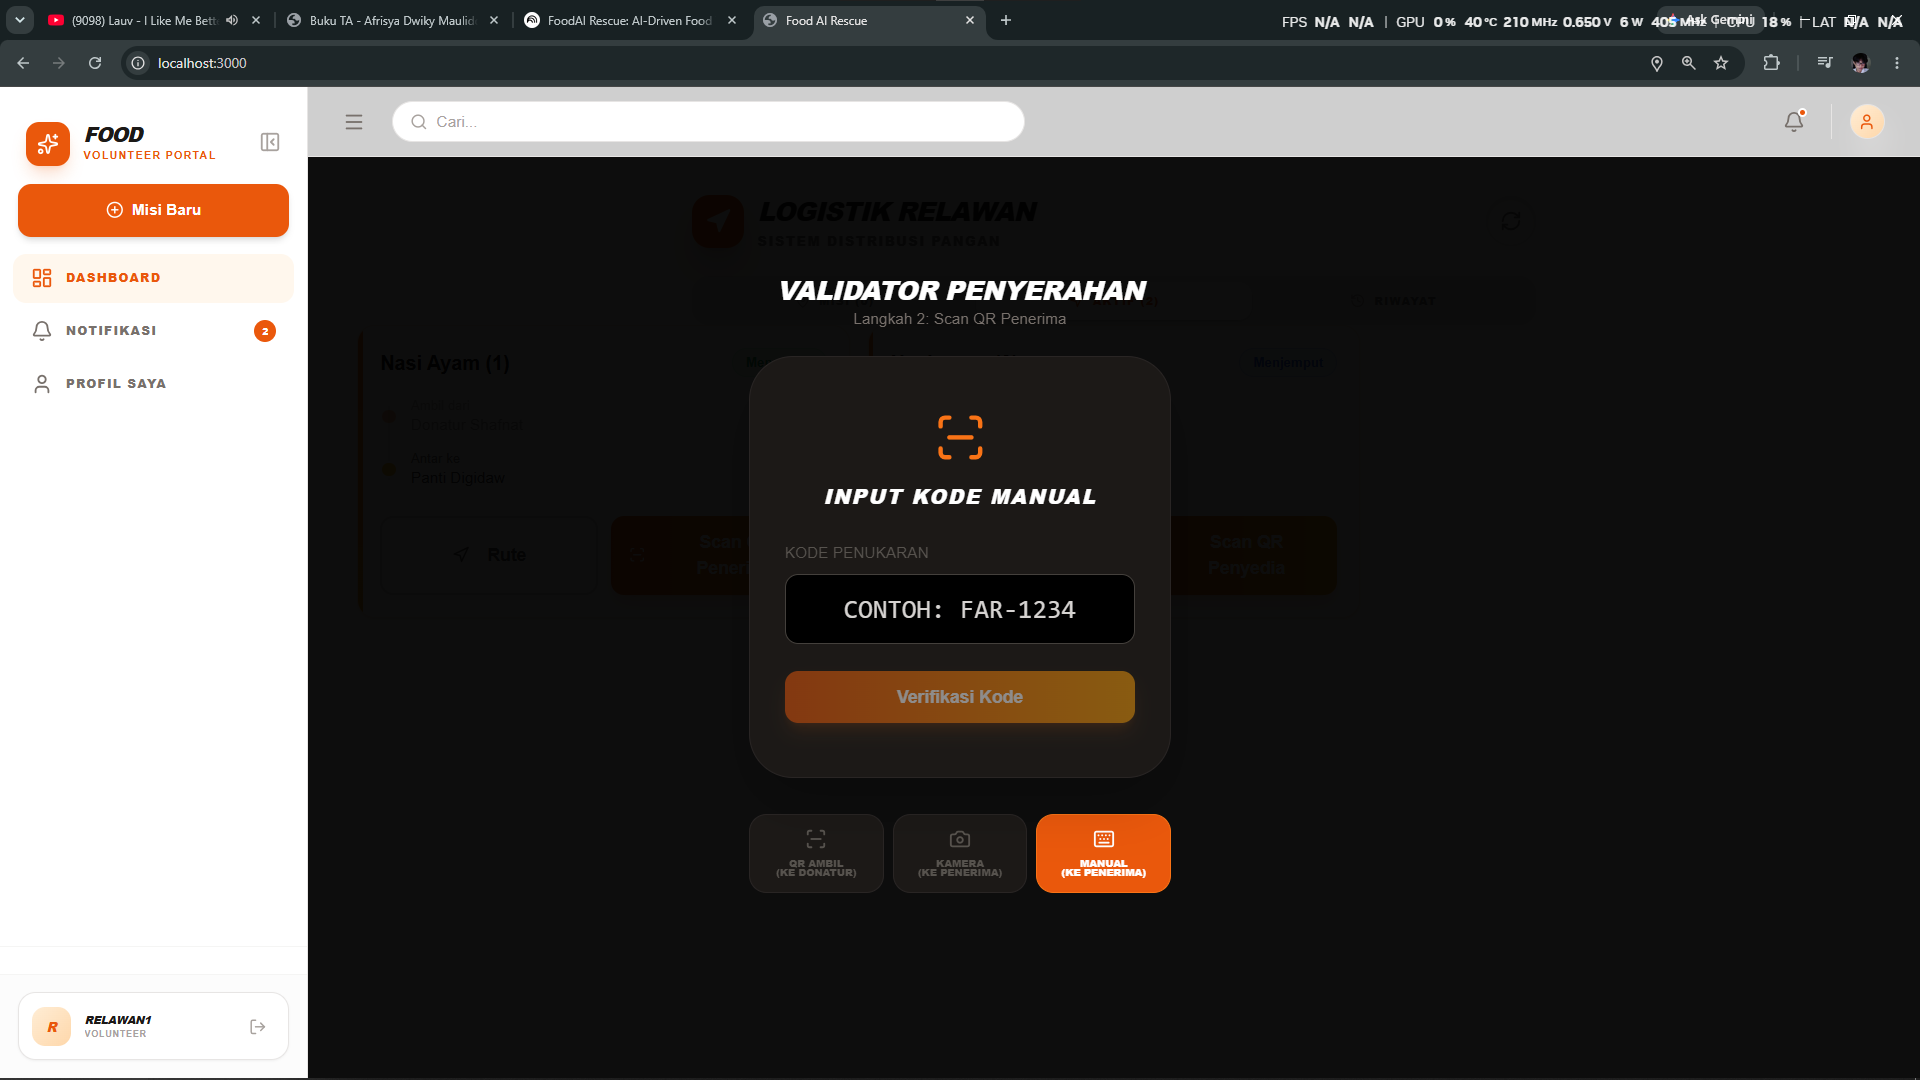
\includegraphics[width=\linewidth]{image/bab4/UserManual/VerifikasiPenerima/2-InputManual.png}
    \caption{Input Kode Manual}
\end{figure}



\section{Pengujian}

Pengujian pada platform FoodAI Rescue dieksekusi menggunakan metode \textit{Black-box Testing}. Metode ini dipilih karena berfokus pada evaluasi fungsionalitas antarmuka sistem---termasuk respons integrasi Kecerdasan Buatan (AI)---tanpa perlu menelusuri struktur internal atau kode sumber programnya. Teknik pengujian yang diterapkan juga disesuaikan dengan karakteristik fitur yang diuji, yang secara spesifik menitikberatkan pada penggunaan teknik \textit{Boundary Value Analysis} (BVA) dan \textit{Equivalence Partitioning} (EP).

Skenario pengujian otomasi dirancang untuk menyimulasikan interaksi dari berbagai target pengguna dengan batasan hak akses yang berbeda di dalam ekosistem aplikasi, meliputi:
\begin{enumerate}[label=\arabic*.]
    \item \textbf{Donatur (Individu dan Korporat)}: Skenario pengujian difokuskan pada simulasi pengunggahan surplus makanan, pencatatan titik jemput logistik, peninjauan Dasbor Dampak Sosial (SROI), serta fungsionalitas verifikasi gambar oleh AI "Polisi Pangan".
    \item \textbf{Penerima Donasi (Fasilitas Sosial/Masyarakat Rentan)}: Skenario pengujian menyimulasikan alur pencarian makanan pada peta ketersediaan (\textit{Radar}) hingga keberhasilan melakukan klaim (\textit{booking}) stok donasi.
    \item \textbf{Relawan (Kurir Logistik)}: Skenario pengujian ditujukan untuk menguji kapabilitas sistem dalam penerimaan misi pengantaran, validasi serah terima melalui pemindaian nirkontak (\textit{scan} QR Code), serta penambahan poin pengalaman (XP) pada sistem gamifikasi.
\end{enumerate}

Pendekatan pengujian berbasis simulasi multikomponen ini bertujuan untuk memastikan bahwa seluruh instrumen sistem mampu mengakomodasi kebutuhan interaksi yang saling berkaitan. Dengan menguji aplikasi dari berbagai sudut pandang otoritas pengguna---mulai dari hulu (penyediaan donasi) hingga hilir (distribusi akhir)---hasil pengujian diharapkan dapat secara komprehensif merefleksikan alur operasional di lapangan, memetakan potensi galat (\textit{bug}) sejak dini, dan menjamin keandalan sistem secara keseluruhan.




\subsection{Skenario Pengujian}
\textbf{a. Skenario 1 – Pembuktian Tujuan 1}

Untuk membuktikan ketercapaian Tujuan 1, yaitu “membangun platform penghubung logistik digital berbasis \textit{Progressive Web App} (PWA) untuk mendistribusikan surplus makanan dari donatur ke fasilitas sosial atau masyarakat rentan secara \textit{real-time} guna mencegah makanan tersebut membusuk menjadi sampah (\textit{food waste})”, maka dilakukan pengujian menggunakan metode \textit{Black-box Testing} dengan teknik \textit{Equivalence Partitioning}. Pengujian ini dieksekusi berdasarkan masukan data pada setiap formulir yang terdapat di antarmuka sistem aplikasi (seperti formulir registrasi, \textit{login}, dan unggah donasi). Setiap parameter masukan akan diuji dan dikelompokkan ke dalam beberapa partisi berdasarkan kesamaan fungsinya, guna memastikan sistem berfungsi dengan benar baik saat menerima data yang bernilai valid maupun tidak valid.

\begin{enumerate}[label=\arabic*.]
    \item \textbf{Validasi Autentikasi Pengguna (Registrasi dan \textit{Login}):}
    \begin{enumerate}[label=\alph*.]
        \item Memastikan pengguna dapat mendaftarkan akun baru dengan melengkapi data yang valid.
        \item Memastikan sistem menolak pendaftaran dan memberikan pesan galat (\textit{error}) apabila pengguna menggunakan alamat email yang sudah terdaftar atau jika konfirmasi kata sandi tidak cocok.
        \item Memastikan sistem memvalidasi kredensial saat \textit{login}, memberikan akses dasbor sesuai peran (\textit{role}) jika data valid, serta menolak akses jika kata sandi atau email yang dimasukkan salah.
    \end{enumerate}
    
    \item \textbf{Validasi Manajemen Unggah Donasi Makanan:}
    \begin{enumerate}[label=\alph*.]
        \item Memastikan donatur (individu maupun korporat) dapat mempublikasikan donasi makanan dengan mengisi kelengkapan formulir dan mengunggah foto yang valid.
        \item Memastikan sistem menggagalkan proses publikasi dan memberikan peringatan apabila donatur mengosongkan \textit{field} yang wajib diisi (seperti nama donasi).
        \item Memastikan sistem memvalidasi input numerik dengan menolak publikasi apabila donatur memasukkan kuantitas porsi donasi yang tidak valid (misalnya mengisi dengan angka 0).
    \end{enumerate}
    
    \item \textbf{Validasi Fungsionalitas Klaim dan Persetujuan Pesanan:}
    \begin{enumerate}[label=\alph*.]
        \item Memastikan pengguna dengan hak akses Penerima dapat mencari dan melakukan klaim pesanan pada makanan yang berstatus tersedia di dasbor mereka.
        \item Memastikan pengguna dengan hak akses Donatur menerima notifikasi pesanan masuk, serta dapat memproses pesanan tersebut dengan melakukan persetujuan (\textit{Terima Request}) agar statusnya berubah menjadi siap diambil, atau melakukan penolakan jika stok bermasalah.
    \end{enumerate}
\end{enumerate}

Guna mendukung kelancaran eksekusi pengujian secara terotomatisasi, skenario pengujian dirancang dengan mengklasifikasikan parameter data uji ke dalam kelas ekuivalen (bernilai valid maupun invalid). Adapun rincian skenario pengujian untuk mengevaluasi fungsionalitas utama sistem (Tujuan 1) dijabarkan pada tabel berikut:

\clearpage
\begin{landscape}
\pagestyle{lscape}
\begin{longtable}{|c|p{3cm}|p{3.5cm}|p{3.5cm}|p{3.5cm}|p{3cm}|p{3cm}|}
\caption{Skenario Pengujian Fitur Utama (Tujuan 1)}
\label{tab:skenario-tujuan1} \\
\hline
\rowcolor{gray!25}
\centering\textbf{Fungsio\-nalitas} & \centering\textbf{ID \textit{Test Case}} & \centering\textbf{Deskripsi/Skenario} & \centering\textbf{Pra Kondisi} & \centering\textbf{Langkah Pengujian} & \centering\textbf{Data Pengujian} & \centering\arraybackslash\textbf{Hasil yang Diharapkan} \\ \hline
\endfirsthead

\hline
\rowcolor{gray!25}
\centering\textbf{Fungsio\-nalitas} & \centering\textbf{ID \textit{Test Case}} & \centering\textbf{Deskripsi/Skenario} & \centering\textbf{Pra Kondisi} & \centering\textbf{Langkah Pengujian} & \centering\textbf{Data Pengujian} & \centering\arraybackslash\textbf{Hasil yang Diharapkan} \\ \hline
\endhead

\hline
\endfoot

\hline
\endlastfoot

% 1. Registrasi
\multirow{3}{2cm}{1. Registrasi} 
& TC1.1 & Pengguna mendaftar dengan data valid & Halaman utama pendaftaran & 1. Klik Daftar Gratis \newline 2. Pilih Peran \newline 3. Isi data lengkap \newline 4. Masukkan OTP & $\bullet$ Nama, email, password valid \newline $\bullet$ OTP sesuai & Registrasi berhasil, masuk ke dashboard \\ \cline{2-7}
& TC1.2 & Pengguna mendaftar dengan email yang sudah digunakan & Halaman utama pendaftaran & 1. Isi email yang terdaftar \newline 2. Klik Daftar & $\bullet$ Email sudah terdaftar & Registrasi gagal, pesan error email digunakan \\ \cline{2-7}
& TC1.3 & Pengguna mendaftar dengan konfirmasi password salah & Halaman utama pendaftaran & 1. Isi form \newline 2. Isi konfirmasi password berbeda & $\bullet$ Konfirmasi pass $\neq$ pass & Registrasi gagal, pesan error password salah \\ \hline

% 2. Login
\multirow{2}{2cm}{2. Login} 
& TC2.1 & Pengguna login dengan kredensial valid & Halaman Login & 1. Masukkan email \newline 2. Masukkan password \newline 3. Klik Masuk & $\bullet$ Email = valid \newline $\bullet$ Pass = valid & Login berhasil, diarahkan ke dashboard \\ \cline{2-7}
& TC2.2 & Pengguna login dengan password salah & Halaman Login & 1. Masukkan email \newline 2. Masukkan password \newline 3. Klik Masuk & $\bullet$ Email = valid \newline $\bullet$ Pass = salah & Login gagal, pesan error kredensial salah \\ \hline

% 3. Input Donasi
\multirow{3}{2cm}{3. Input Donasi} 
& TC3.1 & Donatur menambah donasi dengan data valid & Dashboard Donatur (Stok) & 1. Klik Tambah Donasi \newline 2. Isi kelengkapan \newline 3. Unggah foto \newline 4. Publikasikan & $\bullet$ Data valid, kuantitas $>$ 0, foto valid & Donasi berhasil dipublikasikan \\ \cline{2-7}
& TC3.2 & Donatur mengosongkan \textit{field} wajib & Dashboard Donatur (Stok) & 1. Kosongkan nama donasi \newline 2. Klik Publikasikan & $\bullet$ Nama = null & Publikasi gagal, peringatan field wajib \\ \cline{2-7}
& TC3.3 & Donatur memasukkan kuantitas donasi tidak valid & Dashboard Donatur (Stok) & 1. Isi kuantitas nol \newline 2. Klik Publikasikan & $\bullet$ Kuantitas = 0 & Publikasi gagal, peringatan kuantitas \\ \hline

% 4. Claim Donasi
4. Claim Donasi & TC4.1 & Penerima mengklaim donasi yang tersedia & Dashboard Penerima & 1. Pilih donasi \newline 2. Klik Klaim Sekarang \newline 3. Ya, Yakin & $\bullet$ Stok donasi $>$ 0 & Klaim berhasil, tiket klaim dibuat \\ \hline

% 5. Terima Request
\multirow{2}{2cm}{5. Terima Request} 
& TC5.1 & Donatur menyetujui \textit{request} klaim & Dashboard Donatur (Pesanan) & 1. Detail Pesanan \newline 2. Klik Setujui & $\bullet$ Ada pesanan aktif & Request disetujui, pesanan diproses \\ \cline{2-7}
& TC5.2 & Donatur menolak \textit{request} klaim & Dashboard Donatur (Pesanan) & 1. Detail Pesanan \newline 2. Klik Tolak & $\bullet$ Alasan = stok rusak & Request ditolak, pesanan dibatalkan \\ \hline

\end{longtable}
\pagestyle{fancy}
\end{landscape}
\clearpage

\textbf{2) Cakupan Pengujian Skenario 2}

Pengujian pada skenario ini dirancang untuk membuktikan ketercapaian Tujuan 2 pada aspek keamanan pangan, yakni mengevaluasi keandalan integrasi model Kecerdasan Buatan (Google Gemini Vision API) dalam memvalidasi kelayakan surplus makanan secara visual (\textit{Polisi Pangan}). Mengingat pengujian difokuskan pada alur kerja utama distribusi logistik, evaluasi penerapan AI Generatif untuk kampanye korporat tidak dimasukkan dalam skenario ini. Dengan menerapkan teknik \textit{Equivalence Partitioning} (EP), cakupan pengujian pada modul "Polisi Pangan" meliputi:

\begin{enumerate}[label=\arabic*.]
    \item \textbf{Validasi Visual Kelayakan Donasi Makanan:}
    \begin{enumerate}[label=\alph*.]
        \item Memastikan sistem dapat terintegrasi dengan antarmuka AI untuk memproses unggahan foto makanan dari donatur secara \textit{real-time} saat proses pengisian formulir donasi.
        \item Memastikan algoritma AI mampu menyetujui publikasi donasi (masuk ke dalam katalog ketersediaan) apabila gambar yang diunggah dinilai aman, higienis, dan masuk dalam partisi ekuivalensi data valid.
        \item Memastikan sistem secara otonom dapat mendeteksi, menolak publikasi, dan memberikan peringatan (notifikasi galat) apabila donatur mengunggah gambar yang tidak relevan (misalnya benda mati/objek acak) atau makanan yang secara visual terindikasi tidak layak konsumsi, guna memastikan keamanan pangan bagi penerima di hilir.
    \end{enumerate}
\end{enumerate}

\clearpage
\begin{landscape}
\pagestyle{lscape}
\begin{longtable}{|c|p{3cm}|p{3.5cm}|p{3.5cm}|p{3.5cm}|p{3cm}|p{3cm}|}
\caption{Skenario Pengujian Verifikasi AI (Tujuan 2)}
\label{tab:skenario-tujuan2} \\
\hline
\rowcolor{gray!25}
\centering\textbf{Fungsio\-nalitas} & \centering\textbf{ID \textit{Test Case}} & \centering\textbf{Deskripsi/Skenario} & \centering\textbf{Pra Kondisi} & \centering\textbf{Langkah Pengujian} & \centering\textbf{Data Pengujian} & \centering\arraybackslash\textbf{Hasil yang Diharapkan} \\ \hline
\endfirsthead

\hline
\rowcolor{gray!25}
\centering\textbf{Fungsio\-nalitas} & \centering\textbf{ID \textit{Test Case}} & \centering\textbf{Deskripsi/Skenario} & \centering\textbf{Pra Kondisi} & \centering\textbf{Langkah Pengujian} & \centering\textbf{Data Pengujian} & \centering\arraybackslash\textbf{Hasil yang Diharapkan} \\ \hline
\endhead

\hline
\endfoot

\hline
\endlastfoot

% Audit Foto AI
\multirow{3}{2cm}{Polisi Pangan (Audit AI)} 
& TC-AI.1 & Memvalidasi foto makanan layak konsumsi & Formulir Input Donasi & 1. Unggah foto makanan \newline 2. Sistem memanggil API AI \newline 3. Tampilkan hasil & $\bullet$ Foto makanan utuh dan higienis & AI memberikan skor tinggi, donasi disetujui masuk katalog \\ \cline{2-7}
& TC-AI.2 & Memvalidasi foto objek benda mati & Formulir Input Donasi & 1. Unggah foto objek acak \newline 2. Sistem memanggil API AI \newline 3. Tampilkan hasil & $\bullet$ Foto bukan makanan (objek acak) & AI gagal identifikasi komposisi, publikasi ditolak, muncul galat \\ \cline{2-7}
& TC-AI.3 & Memvalidasi foto makanan tidak layak & Formulir Input Donasi & 1. Unggah foto basi/berjamur \newline 2. Sistem memanggil API AI \newline 3. Tampilkan hasil & $\bullet$ Foto makanan kotor/berjamur & AI mendeteksi ketidaklayakan (skor rendah), publikasi diblokir \\ \hline
\end{longtable}
\pagestyle{fancy}
\end{landscape}
\clearpage

\textbf{c. Skenario 3 – Pembuktian Tujuan 3}

Untuk membuktikan ketercapaian Tujuan 3, yaitu “mengintegrasikan sistem gamifikasi (\textit{leaderboard}), pemindaian Kode QR nirkontak (\textit{contactless}), dan Dasbor Dampak Sosial (SROI) untuk memotivasi partisipasi relawan kurir, mencegah penyalahgunaan klaim ganda saat serah terima di lapangan, dan melacak pencapaian reduksi emisi karbon secara transparan”, maka dilakukan pengujian menggunakan metode \textit{Black-box Testing} dengan teknik \textit{Boundary Value Analysis} (BVA). Pengujian ini merupakan salah satu teknik evaluasi \textit{black-box} yang dirancang secara khusus untuk mengidentifikasi batasan nilai masukan yang krusial dengan menguji titik batas minimum dan maksimum. Pada ekosistem FoodAI Rescue, pengujian ini difokuskan pada batasan nilai numerik yang esensial, seperti batasan input kuantitas porsi donasi makanan (misalnya menginput 0 porsi, angka minus, atau batas maksimal porsi), serta perhitungan poin \textit{Experience} (XP) relawan. Hal ini dilakukan untuk memastikan bahwa logika kalkulasi pada sistem gamifikasi dan dasbor pelacakan dampak sosial (SROI) bekerja secara akurat dan terhindar dari galat manipulasi angka.

\begin{enumerate}[label=\arabic*.]
    \item \textbf{Validasi Manajemen Misi Logistik (Relawan):}
    \begin{enumerate}[label=\alph*.]
        \item Memastikan pengguna dengan hak akses Relawan dapat mengakses dasbor \textit{Missions Board}, melihat detail lokasi, dan berhasil mengklaim (mengambil) misi pengantaran logistik yang berstatus tersedia.
        \item Memastikan relawan dapat membatalkan misi yang telah diambil secara wajar (selama belum diproses lebih lanjut), dan sistem akan secara otomatis mengembalikan misi tersebut ke dalam katalog agar dapat direbut oleh relawan lain.
    \end{enumerate}

    \item \textbf{Validasi Serah Terima Nirkontak (Integrasi Kode QR):}
    \begin{enumerate}[label=\alph*.]
        \item Memastikan relawan mampu memunculkan Kode QR di perangkatnya untuk dipindai oleh donatur, dan memastikan donatur dapat menyetujui serah terima tahap pertama (hulu) menggunakan pemindaian atau input resi manual yang valid.
        \item Memastikan relawan dapat memindai Kode QR milik penerima donasi di titik lokasi tujuan untuk menyelesaikan transaksi distribusi logistik tahap akhir (hilir) apabila kode yang dimasukkan valid.
        \item Memastikan sistem secara tegas menolak, menggagalkan proses serah terima, dan menampilkan peringatan galat (\textit{error}) apabila pengguna (baik donatur maupun relawan) memindai atau memasukkan kode unik buatan yang salah/tidak valid, guna mencegah manipulasi, salah sasaran, maupun klaim ganda.
    \end{enumerate}

    \item \textbf{Validasi Akurasi Gamifikasi dan Dasbor SROI:}
    \begin{enumerate}[label=\alph*.]
        \item Memastikan sistem secara otomatis dan \textit{real-time} menambahkan poin \textit{Experience} (XP) kepada akun relawan sesaat setelah validasi Kode QR penerima dinyatakan sukses, yang memicu pembaruan posisi pada papan peringkat (\textit{Leaderboard}).
        \item Memastikan sistem pada Dasbor Dampak Sosial (SROI) mampu mengakumulasi dan merender grafik kalkulasi konversi secara presisi—dari jumlah porsi makanan yang terselamatkan menjadi data metrik estimasi penghematan air (liter) dan reduksi emisi jejak karbon (kg CO$_2$).
    \end{enumerate}
\end{enumerate}

\clearpage
\begin{landscape}
\pagestyle{lscape}
\begin{longtable}{|c|p{3cm}|p{3.5cm}|p{3.5cm}|p{3.5cm}|p{3cm}|p{3cm}|}
\caption{Skenario Pengujian Operasional Logistik dan Verifikasi (Tujuan 3)}
\label{tab:skenario-tujuan3} \\
\hline
\rowcolor{gray!25}
\centering\textbf{Fungsio\-nalitas} & \centering\textbf{ID \textit{Test Case}} & \centering\textbf{Deskripsi/Skenario} & \centering\textbf{Pra Kondisi} & \centering\textbf{Langkah Pengujian} & \centering\textbf{Data Pengujian} & \centering\arraybackslash\textbf{Hasil yang Diharapkan} \\ \hline
\endfirsthead

\hline
\rowcolor{gray!25}
\centering\textbf{Fungsio\-nalitas} & \centering\textbf{ID \textit{Test Case}} & \centering\textbf{Deskripsi/Skenario} & \centering\textbf{Pra Kondisi} & \centering\textbf{Langkah Pengujian} & \centering\textbf{Data Pengujian} & \centering\arraybackslash\textbf{Hasil yang Diharapkan} \\ \hline
\endhead

\hline
\endfoot

\hline
\endlastfoot

% 6. Ambil Misi
\multirow{2}{2cm}{6. Ambil Misi} 
& TC6.1 & Relawan mengambil misi pengantaran & Dashboard Relawan & 1. Detail Misi \newline 2. Ambil Misi Ini & $\bullet$ Misi status tersedia & Misi berhasil diambil relawan \\ \cline{2-7}
& TC6.3 & Relawan membatalkan misi yang diambil & Dashboard Relawan & 1. Buka misi aktif \newline 2. Batalkan Misi & $\bullet$ Misi belum diproses & Misi berhasil dibatalkan \\ \hline

% 7. Menunjukkan QR
7. Tunjuk QR & TC7.1 & Relawan menampilkan QR ke donatur & Dashboard Relawan & 1. Buka misi aktif \newline 2. Klik QR Ambil & $\bullet$ Relawan di tahap ambil & QR berhasil ditampilkan \\ \hline

% 8. Scan QR
\multirow{2}{2cm}{8. Scan QR} 
& TC8.1 & Donatur verifikasi resi manual relawan dengan benar & Dashboard Donatur & 1. Verifikasi Manual \newline 2. Input resi \newline 3. Verifikasi & $\bullet$ Kode = PICKUP-9800 & Verifikasi berhasil, makanan diserahkan \\ \cline{2-7}
& TC8.3 & Donatur memasukkan resi manual yang salah & Dashboard Donatur & 1. Verifikasi Manual \newline 2. Input resi \newline 3. Verifikasi & $\bullet$ Kode = PICKUP-0000 & Verifikasi gagal, muncul peringatan \\ \hline

% 9. Verifikasi
\multirow{2}{2cm}{9. Verifikasi Penerima} 
& TC9.1 & Relawan memasukkan kode penerima yang benar & Dashboard Relawan & 1. Buka Scan QR Penerima \newline 2. Input kode \newline 3. Verifikasi & $\bullet$ Kode = FAR-5089 & Verifikasi berhasil, misi selesai \\ \cline{2-7}
& TC9.2 & Relawan memasukkan kode penerima yang salah & Dashboard Relawan & 1. Buka Scan QR Penerima \newline 2. Input kode \newline 3. Verifikasi & $\bullet$ Kode = FAR-0000 & Verifikasi gagal, peringatan kode salah \\ \hline
\end{longtable}
\pagestyle{fancy}
\end{landscape}
\clearpage


\subsection{Hasil Pengujian}

Tahapan ini memaparkan hasil evaluasi dari eksekusi rancangan pengujian (\textit{test case}) yang telah disusun sebelumnya. Pengujian fungsionalitas sistem dieksekusi menggunakan perangkat lunak otomasi Katalon Studio. Hasil aktual dari respons antarmuka dan sistem \textit{backend} dikomparasikan dengan ekspektasi hasil untuk menentukan status keberhasilan. Skenario dinyatakan \textbf{\textit{Pass}} (Berhasil) apabila respons sistem sejalan dengan ekspektasi, dan dinyatakan \textbf{\textit{Failed}} (Gagal) apabila ditemukan galat (\textit{bug}) atau ketidaksesuaian validasi pada sistem.

\textbf{a. Hasil Pengujian Skenario 1 (Pembuktian Tujuan 1)}

Pengujian pada tahap ini difokuskan pada alur kerja utama aplikasi (\textit{core business flow}), mulai dari pendaftaran akun, autentikasi, penyediaan donasi, hingga proses klaim pesanan.

\begin{table}[H]
\centering
\caption{Hasil Pengujian Fitur Utama (Tujuan 1)}
\label{tab:hasil-tujuan1}
\begin{tabularx}{\textwidth}{|c|L|L|L|c|}
\hline
\rowcolor{gray!25}
\textbf{ID} & \textbf{Fitur yang Diuji} & \textbf{Langkah Pengujian (Simulasi Sistem)} & \textbf{Hasil Aktual Sistem} & \textbf{Status} \\ \hline
\textbf{TC1.1} & Registrasi (Valid) & Sistem menyimulasikan pengisian formulir daftar (nama, email baru, \textit{password}, nomor WA) dan menekan tombol "Daftar". & Akun berhasil dibuat dan pengguna langsung diarahkan ke \textit{Dashboard}. & \textbf{Pass} \\ \hline
\textbf{TC1.2} & Registrasi (Email Duplikat) & Sistem menyimulasikan pendaftaran menggunakan alamat email yang sudah pernah terdaftar di basis data. & Sistem menolak pendaftaran dan memunculkan peringatan "Email sudah digunakan". & \textbf{Pass} \\ \hline
\textbf{TC1.3} & Registrasi (Sandi Tidak Cocok) & Sistem menginputkan kata sandi utama dan konfirmasi kata sandi yang berbeda. & Sistem menggagalkan proses dan memunculkan peringatan validasi \textit{password}. & \textbf{Pass} \\ \hline
\textbf{TC2.1} & Login (Valid) & Sistem menginputkan email dan kata sandi yang benar, lalu menekan tombol "Masuk". & Autentikasi berhasil, pengguna dialihkan ke Dasbor sesuai perannya (\textit{Role}). & \textbf{Pass} \\ \hline
\textbf{TC2.2} & Login (Invalid) & Sistem menginputkan kombinasi email atau kata sandi yang salah/tidak terdaftar. & Autentikasi ditolak, muncul peringatan galat "Kredensial salah". & \textbf{Pass} \\ \hline
\textbf{TC3.1} & Input Donasi (Valid) & Donatur mengisi lengkap data makanan, mengunggah foto, dan memublikasikannya. & Data terkirim ke \textit{backend}, divalidasi, dan donasi berhasil masuk ke katalog. & \textbf{Pass} \\ \hline
\textbf{TC3.2} & Input Donasi (Field Kosong) & Donatur sengaja mengosongkan \textit{field} wajib (seperti nama donasi) dan mencoba menyimpan. & Sistem \textbf{gagal} memblokir proses penyimpanan, peringatan validasi tidak muncul secara tepat. & \textbf{Failed} \\ \hline
\textbf{TC3.3} & Input Donasi (Kuantitas Nol) & Donatur memasukkan angka 0 pada jumlah porsi makanan. & Sistem \textbf{gagal} menolak input batas bawah (BVA), sehingga donasi dengan porsi 0 lolos. & \textbf{Failed} \\ \hline
\textbf{TC4.1} & Klaim Donasi & Penerima mencari makanan di katalog, mengatur lokasi, dan menekan "Klaim Sekarang". & Transaksi klaim berhasil dibuat dan status stok makanan terkunci. & \textbf{Pass} \\ \hline
\textbf{TC5.1} & Terima Pesanan & Donatur membuka riwayat pesanan masuk dan menekan tombol "Setujui". & Status pesanan diperbarui menjadi "Siap Diambil" oleh sistem. & \textbf{Pass} \\ \hline
\textbf{TC5.2} & Tolak Pesanan & Donatur menekan tombol "Tolak" karena alasan stok bermasalah. & Pesanan berhasil dibatalkan dan dikembalikan statusnya. & \textbf{Pass} \\ \hline
\end{tabularx}
\end{table}

\textbf{b. Hasil Pengujian Skenario 2 (Pembuktian Tujuan 2)}

Pengujian ini berfokus pada ketangguhan validasi integrasi \textit{Google Gemini Vision API} yang bertindak sebagai "Polisi Pangan" saat donatur mengunggah foto makanan.

\begin{table}[H]
\centering
\caption{Hasil Pengujian Verifikasi AI (Tujuan 2)}
\label{tab:hasil-tujuan2}
\begin{tabularx}{\textwidth}{|c|L|L|L|c|}
\hline
\rowcolor{gray!25}
\textbf{ID} & \textbf{Fitur yang Diuji} & \textbf{Langkah Pengujian (Simulasi Sistem)} & \textbf{Hasil Aktual Sistem} & \textbf{Status} \\ \hline
\textbf{TC-AI.1} & Audit AI (Foto Valid) & Mengunggah foto makanan utuh dan menekan tombol "Lanjut ke Foto Audit AI". & AI mengekstraksi skor keamanan tinggi dan menyetujui publikasi donasi. & \textbf{Pass} \\ \hline
\textbf{TC-AI.2} & Audit AI (Bukan Makanan) & Mengunggah foto objek acak (benda mati) untuk menguji \textit{Clever Hans effect}. & AI gagal mendeteksi komposisi makanan dan menolak proses publikasi. & \textbf{Pass} \\ \hline
\textbf{TC-AI.3} & Audit AI (Tidak Layak) & Mengunggah foto makanan berjamur/kotor. & AI memberikan skor keamanan rendah dan memblokir publikasi. & \textbf{Pass} \\ \hline
\end{tabularx}
\end{table}

\textit{(Catatan: Kode TC-AI.x ditambahkan khusus untuk Buku TA guna menjelaskan apa yang terjadi di balik layar saat skrip Katalon Anda menekan tombol "Lanjut ke Foto Audit AI" pada skenario input donasi).}

\textbf{c. Hasil Pengujian Skenario 3 (Pembuktian Tujuan 3)}

Pengujian ini mengevaluasi keandalan operasional logistik di lapangan, keamanan sistem pindai Kode QR secara nirkontak, serta pemicu (\textit{trigger}) ke sistem poin gamifikasi.

\begin{table}[H]
\centering
\caption{Hasil Pengujian Logistik dan Verifikasi (Tujuan 3)}
\label{tab:hasil-tujuan3}
\begin{tabularx}{\textwidth}{|c|L|L|L|c|}
\hline
\rowcolor{gray!25}
\textbf{ID} & \textbf{Fitur yang Diuji} & \textbf{Langkah Pengujian (Simulasi Sistem)} & \textbf{Hasil Aktual Sistem} & \textbf{Status} \\ \hline
\textbf{TC6.1} & Ambil Misi Logistik & Relawan membuka \textit{Missions Board} dan menekan tombol "Ambil Misi Ini". & Misi berhasil ditugaskan ke relawan dan rute penjemputan ditampilkan. & \textbf{Pass} \\ \hline
\textbf{TC6.2} & Batal Misi & Relawan menekan tombol "Batalkan Misi" sebelum diproses lebih lanjut. & Misi dilepas dan dikembalikan ke daftar agar bisa diambil relawan lain. & \textbf{Pass} \\ \hline
\textbf{TC7.1} & Generate QR Code & Relawan menekan tombol "QR Ambil" saat tiba di lokasi donatur. & Sistem berhasil merender Kode QR unik milik relawan di layar. & \textbf{Pass} \\ \hline
\textbf{TC8.1} & Verifikasi Penjemputan (Valid) & Donatur memindai atau menginput resi nirkontak relawan dengan kode yang \textbf{benar}. & Verifikasi sukses, makanan sah diserahkan ke relawan, misi berlanjut. & \textbf{Pass} \\ \hline
\textbf{TC8.3} & Verifikasi Penjemputan (Invalid) & Donatur memasukkan resi dengan kode acak/salah (misal: \texttt{PICKUP-0000}). & Sistem menolak serah terima dan memunculkan peringatan kode salah. & \textbf{Pass} \\ \hline
\textbf{TC9.1} & Verifikasi Pengantaran (Valid) & Relawan tiba di lokasi tujuan dan menginput kode unik penerima yang \textbf{benar}. & Verifikasi sukses, transaksi selesai (\textit{Completed}), dan poin Gamifikasi bertambah. & \textbf{Pass} \\ \hline
\textbf{TC9.2} & Verifikasi Pengantaran (Invalid) & Relawan memasukkan kode penerima yang salah (misal: \texttt{FAR-0000}). & Verifikasi gagal, sistem mencegah penyelesaian misi untuk menghindari salah sasaran. & \textbf{Pass} \\ \hline
\end{tabularx}
\end{table}


